\documentclass[]{book}
\usepackage{lmodern}
\usepackage{amssymb,amsmath}
\usepackage{ifxetex,ifluatex}
\usepackage{fixltx2e} % provides \textsubscript
\ifnum 0\ifxetex 1\fi\ifluatex 1\fi=0 % if pdftex
  \usepackage[T1]{fontenc}
  \usepackage[utf8]{inputenc}
\else % if luatex or xelatex
  \ifxetex
    \usepackage{mathspec}
  \else
    \usepackage{fontspec}
  \fi
  \defaultfontfeatures{Ligatures=TeX,Scale=MatchLowercase}
\fi
% use upquote if available, for straight quotes in verbatim environments
\IfFileExists{upquote.sty}{\usepackage{upquote}}{}
% use microtype if available
\IfFileExists{microtype.sty}{%
\usepackage{microtype}
\UseMicrotypeSet[protrusion]{basicmath} % disable protrusion for tt fonts
}{}
\usepackage{hyperref}
\hypersetup{unicode=true,
            pdftitle={A Minimal rTorch Tutorial},
            pdfauthor={Alfonso R. Reyes},
            pdfborder={0 0 0},
            breaklinks=true}
\urlstyle{same}  % don't use monospace font for urls
\usepackage{natbib}
\bibliographystyle{apalike}
\usepackage{color}
\usepackage{fancyvrb}
\newcommand{\VerbBar}{|}
\newcommand{\VERB}{\Verb[commandchars=\\\{\}]}
\DefineVerbatimEnvironment{Highlighting}{Verbatim}{commandchars=\\\{\}}
% Add ',fontsize=\small' for more characters per line
\usepackage{framed}
\definecolor{shadecolor}{RGB}{248,248,248}
\newenvironment{Shaded}{\begin{snugshade}}{\end{snugshade}}
\newcommand{\AlertTok}[1]{\textcolor[rgb]{0.94,0.16,0.16}{#1}}
\newcommand{\AnnotationTok}[1]{\textcolor[rgb]{0.56,0.35,0.01}{\textbf{\textit{#1}}}}
\newcommand{\AttributeTok}[1]{\textcolor[rgb]{0.77,0.63,0.00}{#1}}
\newcommand{\BaseNTok}[1]{\textcolor[rgb]{0.00,0.00,0.81}{#1}}
\newcommand{\BuiltInTok}[1]{#1}
\newcommand{\CharTok}[1]{\textcolor[rgb]{0.31,0.60,0.02}{#1}}
\newcommand{\CommentTok}[1]{\textcolor[rgb]{0.56,0.35,0.01}{\textit{#1}}}
\newcommand{\CommentVarTok}[1]{\textcolor[rgb]{0.56,0.35,0.01}{\textbf{\textit{#1}}}}
\newcommand{\ConstantTok}[1]{\textcolor[rgb]{0.00,0.00,0.00}{#1}}
\newcommand{\ControlFlowTok}[1]{\textcolor[rgb]{0.13,0.29,0.53}{\textbf{#1}}}
\newcommand{\DataTypeTok}[1]{\textcolor[rgb]{0.13,0.29,0.53}{#1}}
\newcommand{\DecValTok}[1]{\textcolor[rgb]{0.00,0.00,0.81}{#1}}
\newcommand{\DocumentationTok}[1]{\textcolor[rgb]{0.56,0.35,0.01}{\textbf{\textit{#1}}}}
\newcommand{\ErrorTok}[1]{\textcolor[rgb]{0.64,0.00,0.00}{\textbf{#1}}}
\newcommand{\ExtensionTok}[1]{#1}
\newcommand{\FloatTok}[1]{\textcolor[rgb]{0.00,0.00,0.81}{#1}}
\newcommand{\FunctionTok}[1]{\textcolor[rgb]{0.00,0.00,0.00}{#1}}
\newcommand{\ImportTok}[1]{#1}
\newcommand{\InformationTok}[1]{\textcolor[rgb]{0.56,0.35,0.01}{\textbf{\textit{#1}}}}
\newcommand{\KeywordTok}[1]{\textcolor[rgb]{0.13,0.29,0.53}{\textbf{#1}}}
\newcommand{\NormalTok}[1]{#1}
\newcommand{\OperatorTok}[1]{\textcolor[rgb]{0.81,0.36,0.00}{\textbf{#1}}}
\newcommand{\OtherTok}[1]{\textcolor[rgb]{0.56,0.35,0.01}{#1}}
\newcommand{\PreprocessorTok}[1]{\textcolor[rgb]{0.56,0.35,0.01}{\textit{#1}}}
\newcommand{\RegionMarkerTok}[1]{#1}
\newcommand{\SpecialCharTok}[1]{\textcolor[rgb]{0.00,0.00,0.00}{#1}}
\newcommand{\SpecialStringTok}[1]{\textcolor[rgb]{0.31,0.60,0.02}{#1}}
\newcommand{\StringTok}[1]{\textcolor[rgb]{0.31,0.60,0.02}{#1}}
\newcommand{\VariableTok}[1]{\textcolor[rgb]{0.00,0.00,0.00}{#1}}
\newcommand{\VerbatimStringTok}[1]{\textcolor[rgb]{0.31,0.60,0.02}{#1}}
\newcommand{\WarningTok}[1]{\textcolor[rgb]{0.56,0.35,0.01}{\textbf{\textit{#1}}}}
\usepackage{longtable,booktabs}
\usepackage{graphicx,grffile}
\makeatletter
\def\maxwidth{\ifdim\Gin@nat@width>\linewidth\linewidth\else\Gin@nat@width\fi}
\def\maxheight{\ifdim\Gin@nat@height>\textheight\textheight\else\Gin@nat@height\fi}
\makeatother
% Scale images if necessary, so that they will not overflow the page
% margins by default, and it is still possible to overwrite the defaults
% using explicit options in \includegraphics[width, height, ...]{}
\setkeys{Gin}{width=\maxwidth,height=\maxheight,keepaspectratio}
\IfFileExists{parskip.sty}{%
\usepackage{parskip}
}{% else
\setlength{\parindent}{0pt}
\setlength{\parskip}{6pt plus 2pt minus 1pt}
}
\setlength{\emergencystretch}{3em}  % prevent overfull lines
\providecommand{\tightlist}{%
  \setlength{\itemsep}{0pt}\setlength{\parskip}{0pt}}
\setcounter{secnumdepth}{5}
% Redefines (sub)paragraphs to behave more like sections
\ifx\paragraph\undefined\else
\let\oldparagraph\paragraph
\renewcommand{\paragraph}[1]{\oldparagraph{#1}\mbox{}}
\fi
\ifx\subparagraph\undefined\else
\let\oldsubparagraph\subparagraph
\renewcommand{\subparagraph}[1]{\oldsubparagraph{#1}\mbox{}}
\fi

%%% Use protect on footnotes to avoid problems with footnotes in titles
\let\rmarkdownfootnote\footnote%
\def\footnote{\protect\rmarkdownfootnote}

%%% Change title format to be more compact
\usepackage{titling}

% Create subtitle command for use in maketitle
\providecommand{\subtitle}[1]{
  \posttitle{
    \begin{center}\large#1\end{center}
    }
}

\setlength{\droptitle}{-2em}

  \title{A Minimal rTorch Tutorial}
    \pretitle{\vspace{\droptitle}\centering\huge}
  \posttitle{\par}
    \author{Alfonso R. Reyes}
    \preauthor{\centering\large\emph}
  \postauthor{\par}
      \predate{\centering\large\emph}
  \postdate{\par}
    \date{2019-08-10}

\usepackage{booktabs}

\begin{document}
\maketitle

{
\setcounter{tocdepth}{1}
\tableofcontents
}
\hypertarget{prerequisites}{%
\chapter{Prerequisites}\label{prerequisites}}

You need two things to get \texttt{rTorch} working:

\begin{enumerate}
\def\labelenumi{\arabic{enumi}.}
\item
  Python \href{}{Anaconda} installed.
\item
  Install \texttt{rTorch} from CRAN or GitHub.
\end{enumerate}

The \textbf{rTorch} package can be installed from CRAN or Github:

\begin{Shaded}
\begin{Highlighting}[]
\KeywordTok{install.packages}\NormalTok{(}\StringTok{"rTorch"}\NormalTok{)}
\CommentTok{# or the development version}
\CommentTok{# devtools::install_github("f0nzie/rTorch")}
\end{Highlighting}
\end{Shaded}

\begin{quote}
Note. It is not mandatory to have a previously Python environment created with Anaconda where PyTorch and TorchVision have been installed. You could also installed directly from the R console in similar fashion as \href{}{TensorFlow} using the function \texttt{install\_pytorch}.
\end{quote}

To compile this example to PDF, you need XeLaTeX. You are recommended to install TinyTeX (which includes XeLaTeX): \url{https://yihui.name/tinytex/}.

\hypertarget{intro}{%
\chapter{Introduction}\label{intro}}

You can label chapter and section titles using \texttt{\{\#label\}} after them, e.g., we can reference Chapter \ref{intro}. If you do not manually label them, there will be automatic labels anyway, e.g., Chapter @ref(linear\_algebra).

Figures and tables with captions will be placed in \texttt{figure} and \texttt{table} environments, respectively.

\begin{Shaded}
\begin{Highlighting}[]
\KeywordTok{par}\NormalTok{(}\DataTypeTok{mar =} \KeywordTok{c}\NormalTok{(}\DecValTok{4}\NormalTok{, }\DecValTok{4}\NormalTok{, }\FloatTok{.1}\NormalTok{, }\FloatTok{.1}\NormalTok{))}
\KeywordTok{plot}\NormalTok{(pressure, }\DataTypeTok{type =} \StringTok{'b'}\NormalTok{, }\DataTypeTok{pch =} \DecValTok{19}\NormalTok{)}
\end{Highlighting}
\end{Shaded}

\begin{figure}

{\centering 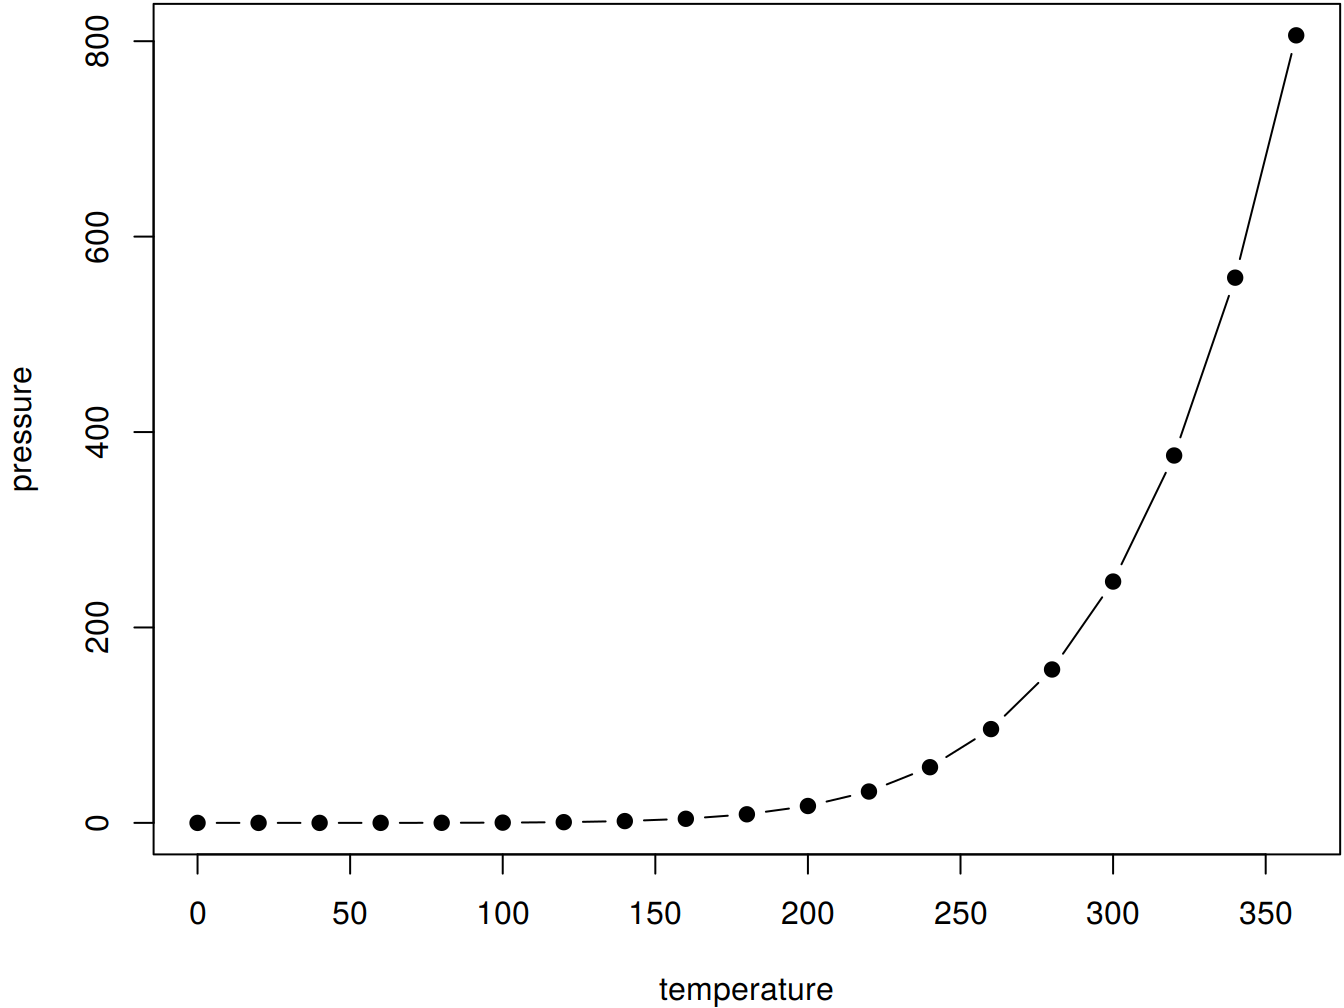
\includegraphics[width=0.8\linewidth]{rtorch-book_files/figure-latex/nice-fig-1} 

}

\caption{Here is a nice figure!}\label{fig:nice-fig}
\end{figure}

Reference a figure by its code chunk label with the \texttt{fig:} prefix, e.g., see Figure \ref{fig:nice-fig}. Similarly, you can reference tables generated from \texttt{knitr::kable()}, e.g., see Table \ref{tab:nice-tab}.

\begin{Shaded}
\begin{Highlighting}[]
\NormalTok{knitr}\OperatorTok{::}\KeywordTok{kable}\NormalTok{(}
  \KeywordTok{head}\NormalTok{(iris, }\DecValTok{20}\NormalTok{), }\DataTypeTok{caption =} \StringTok{'Here is a nice table!'}\NormalTok{,}
  \DataTypeTok{booktabs =} \OtherTok{TRUE}
\NormalTok{)}
\end{Highlighting}
\end{Shaded}

\begin{table}[t]

\caption{\label{tab:nice-tab}Here is a nice table!}
\centering
\begin{tabular}{rrrrl}
\toprule
Sepal.Length & Sepal.Width & Petal.Length & Petal.Width & Species\\
\midrule
5.1 & 3.5 & 1.4 & 0.2 & setosa\\
4.9 & 3.0 & 1.4 & 0.2 & setosa\\
4.7 & 3.2 & 1.3 & 0.2 & setosa\\
4.6 & 3.1 & 1.5 & 0.2 & setosa\\
5.0 & 3.6 & 1.4 & 0.2 & setosa\\
\addlinespace
5.4 & 3.9 & 1.7 & 0.4 & setosa\\
4.6 & 3.4 & 1.4 & 0.3 & setosa\\
5.0 & 3.4 & 1.5 & 0.2 & setosa\\
4.4 & 2.9 & 1.4 & 0.2 & setosa\\
4.9 & 3.1 & 1.5 & 0.1 & setosa\\
\addlinespace
5.4 & 3.7 & 1.5 & 0.2 & setosa\\
4.8 & 3.4 & 1.6 & 0.2 & setosa\\
4.8 & 3.0 & 1.4 & 0.1 & setosa\\
4.3 & 3.0 & 1.1 & 0.1 & setosa\\
5.8 & 4.0 & 1.2 & 0.2 & setosa\\
\addlinespace
5.7 & 4.4 & 1.5 & 0.4 & setosa\\
5.4 & 3.9 & 1.3 & 0.4 & setosa\\
5.1 & 3.5 & 1.4 & 0.3 & setosa\\
5.7 & 3.8 & 1.7 & 0.3 & setosa\\
5.1 & 3.8 & 1.5 & 0.3 & setosa\\
\bottomrule
\end{tabular}
\end{table}

You can write citations, too. For example, we are using the \textbf{bookdown} package \citep{R-bookdown} in this sample book, which was built on top of R Markdown and \textbf{knitr} \citep{xie2015}.

\hypertarget{installation}{%
\section{Installation}\label{installation}}

\texttt{rTorch} is available in GitHub only at this moment.

Install \texttt{rTorch} with:

\texttt{devtools::install\_github("f0nzie/rTorch")}

Before start running \texttt{rTorch}, install a Python Anaconda environment first.

\begin{enumerate}
\def\labelenumi{\arabic{enumi}.}
\item
  Create a conda environment with \texttt{conda\ create\ -n\ myenv\ python=3.7}
\item
  Activate the new environment with \texttt{conda\ activate\ myenv}
\item
  Install PyTorch related packages with:
\end{enumerate}

\texttt{conda\ install\ python=3.6.6\ pytorch-cpu\ torchvision-cpu\ matplotlib\ pandas\ -c\ pytorch}

Now, you can load \texttt{rTorch} in R or RStudio.

The automatic installation, like in \texttt{rtensorflow}, may be available later.

\textbf{Note.} \texttt{matplotlib} and \texttt{pandas} are not really necessary, but I was asked if \texttt{matplotlib} or \texttt{pandas} would in PyTorch, that I decided to put them for testing and experimentation. They both work.

\hypertarget{matrices-and-linear-algebra}{%
\section{Matrices and Linear Algebra}\label{matrices-and-linear-algebra}}

There are five major type of Tensors in PyTorch

\begin{Shaded}
\begin{Highlighting}[]
\KeywordTok{library}\NormalTok{(rTorch)}

\NormalTok{bt <-}\StringTok{ }\NormalTok{torch}\OperatorTok{$}\KeywordTok{ByteTensor}\NormalTok{(3L, 3L)}
\NormalTok{ft <-}\StringTok{ }\NormalTok{torch}\OperatorTok{$}\KeywordTok{FloatTensor}\NormalTok{(3L, 3L)}
\NormalTok{dt <-}\StringTok{ }\NormalTok{torch}\OperatorTok{$}\KeywordTok{DoubleTensor}\NormalTok{(3L, 3L)}
\NormalTok{lt <-}\StringTok{ }\NormalTok{torch}\OperatorTok{$}\KeywordTok{LongTensor}\NormalTok{(3L, 3L)}
\NormalTok{Bt <-}\StringTok{ }\NormalTok{torch}\OperatorTok{$}\KeywordTok{BoolTensor}\NormalTok{(5L, 5L)}

\NormalTok{ft}
\end{Highlighting}
\end{Shaded}

\begin{verbatim}
## tensor([[-6.3276e-21,  4.5744e-41, -6.3276e-21],
##         [ 4.5744e-41,  4.1075e+18,  9.2737e-41],
##         [ 2.1163e-37,  2.1214e-37,  1.9304e-37]])
\end{verbatim}

\begin{Shaded}
\begin{Highlighting}[]
\NormalTok{dt}
\end{Highlighting}
\end{Shaded}

\begin{verbatim}
## tensor([[6.9272e-310, 4.6816e-310, 4.6816e-310],
##         [6.9272e-310, 8.3991e-323,  0.0000e+00],
##         [4.6816e-310, 4.6816e-310, 4.6816e-310]], dtype=torch.float64)
\end{verbatim}

\begin{Shaded}
\begin{Highlighting}[]
\NormalTok{Bt}
\end{Highlighting}
\end{Shaded}

\begin{verbatim}
## tensor([[ True,  True,  True,  True,  True],
##         [ True, False, False,  True,  True],
##         [ True,  True,  True,  True, False],
##         [False,  True,  True,  True,  True],
##         [ True,  True, False, False,  True]], dtype=torch.bool)
\end{verbatim}

A 4D tensor like in MNIST hand-written digits recognition dataset:

\begin{Shaded}
\begin{Highlighting}[]
\NormalTok{mnist_4d <-}\StringTok{ }\NormalTok{torch}\OperatorTok{$}\KeywordTok{FloatTensor}\NormalTok{(60000L, 3L, 28L, 28L)}

\CommentTok{# size}
\NormalTok{mnist_4d}\OperatorTok{$}\KeywordTok{size}\NormalTok{()}
\end{Highlighting}
\end{Shaded}

\begin{verbatim}
## torch.Size([60000, 3, 28, 28])
\end{verbatim}

\begin{Shaded}
\begin{Highlighting}[]
\CommentTok{# length}
\KeywordTok{length}\NormalTok{(mnist_4d)}
\end{Highlighting}
\end{Shaded}

\begin{verbatim}
## [1] 141120000
\end{verbatim}

\begin{Shaded}
\begin{Highlighting}[]
\CommentTok{# shape, like in numpy}
\NormalTok{mnist_4d}\OperatorTok{$}\NormalTok{shape}
\end{Highlighting}
\end{Shaded}

\begin{verbatim}
## torch.Size([60000, 3, 28, 28])
\end{verbatim}

\begin{Shaded}
\begin{Highlighting}[]
\CommentTok{# number of elements}
\NormalTok{mnist_4d}\OperatorTok{$}\KeywordTok{numel}\NormalTok{()}
\end{Highlighting}
\end{Shaded}

\begin{verbatim}
## [1] 141120000
\end{verbatim}

A 3D tensor:

\begin{Shaded}
\begin{Highlighting}[]
\NormalTok{ft3d <-}\StringTok{ }\NormalTok{torch}\OperatorTok{$}\KeywordTok{FloatTensor}\NormalTok{(4L, 3L, 2L)}
\NormalTok{ft3d}
\end{Highlighting}
\end{Shaded}

\begin{verbatim}
## tensor([[[2.5223e-44, 0.0000e+00],
##          [0.0000e+00, 0.0000e+00],
##          [2.3557e+30, 3.0915e-41]],
## 
##         [[2.3557e+30, 3.0915e-41],
##          [2.3557e+30, 3.0915e-41],
##          [1.1412e+30, 3.0915e-41]],
## 
##         [[1.1412e+30, 3.0915e-41],
##          [1.1412e+30, 3.0915e-41],
##          [1.1412e+30, 3.0915e-41]],
## 
##         [[1.1412e+30, 3.0915e-41],
##          [1.1412e+30, 3.0915e-41],
##          [1.1412e+30, 3.0915e-41]]])
\end{verbatim}

\begin{Shaded}
\begin{Highlighting}[]
\CommentTok{# get first element in a tensor}
\NormalTok{ft3d[}\DecValTok{1}\NormalTok{, }\DecValTok{1}\NormalTok{, }\DecValTok{1}\NormalTok{]}
\end{Highlighting}
\end{Shaded}

\begin{verbatim}
## tensor(2.5223e-44)
\end{verbatim}

\begin{Shaded}
\begin{Highlighting}[]
\NormalTok{bt}
\end{Highlighting}
\end{Shaded}

\begin{verbatim}
## tensor([[160,  12, 239],
##         [157, 132, 127],
##         [  0,   0, 160]], dtype=torch.uint8)
\end{verbatim}

\begin{Shaded}
\begin{Highlighting}[]
\CommentTok{# [torch.ByteTensor of size 3x3]}
\end{Highlighting}
\end{Shaded}

\begin{Shaded}
\begin{Highlighting}[]
\NormalTok{ft}
\end{Highlighting}
\end{Shaded}

\begin{verbatim}
## tensor([[-6.3276e-21,  4.5744e-41, -6.3276e-21],
##         [ 4.5744e-41,  4.1075e+18,  9.2737e-41],
##         [ 2.1163e-37,  2.1214e-37,  1.9304e-37]])
\end{verbatim}

\begin{Shaded}
\begin{Highlighting}[]
\CommentTok{# [torch.FloatTensor of size 3x3]}
\end{Highlighting}
\end{Shaded}

\begin{Shaded}
\begin{Highlighting}[]
\CommentTok{# create a tensor with a value}
\NormalTok{torch}\OperatorTok{$}\KeywordTok{full}\NormalTok{(}\KeywordTok{list}\NormalTok{(2L, 3L), }\FloatTok{3.141592}\NormalTok{)}
\end{Highlighting}
\end{Shaded}

\begin{verbatim}
## tensor([[3.1416, 3.1416, 3.1416],
##         [3.1416, 3.1416, 3.1416]])
\end{verbatim}

\hypertarget{lessons-learned}{%
\chapter{Lessons Learned}\label{lessons-learned}}

Here is a review of existing methods.

\begin{Shaded}
\begin{Highlighting}[]
\KeywordTok{library}\NormalTok{(rTorch)}
\end{Highlighting}
\end{Shaded}

\hypertarget{enumeration}{%
\section{Enumeration}\label{enumeration}}

\begin{Shaded}
\begin{Highlighting}[]
\NormalTok{x_train =}\StringTok{ }\KeywordTok{array}\NormalTok{(}\KeywordTok{c}\NormalTok{(}\FloatTok{3.3}\NormalTok{, }\FloatTok{4.4}\NormalTok{, }\FloatTok{5.5}\NormalTok{, }\FloatTok{6.71}\NormalTok{, }\FloatTok{6.93}\NormalTok{, }\FloatTok{4.168}\NormalTok{, }
                  \FloatTok{9.779}\NormalTok{, }\FloatTok{6.182}\NormalTok{, }\FloatTok{7.59}\NormalTok{, }\FloatTok{2.167}\NormalTok{, }\FloatTok{7.042}\NormalTok{,}
                  \FloatTok{10.791}\NormalTok{, }\FloatTok{5.313}\NormalTok{, }\FloatTok{7.997}\NormalTok{, }\FloatTok{3.1}\NormalTok{), }\DataTypeTok{dim =} \KeywordTok{c}\NormalTok{(}\DecValTok{15}\NormalTok{,}\DecValTok{1}\NormalTok{))}

\NormalTok{x_train <-}\StringTok{ }\KeywordTok{r_to_py}\NormalTok{(x_train)}
\NormalTok{x_train =}\StringTok{ }\NormalTok{torch}\OperatorTok{$}\KeywordTok{from_numpy}\NormalTok{(x_train)         }\CommentTok{# convert to tensor}
\NormalTok{x_train =}\StringTok{ }\NormalTok{x_train}\OperatorTok{$}\KeywordTok{type}\NormalTok{(torch}\OperatorTok{$}\NormalTok{FloatTensor)   }\CommentTok{# make it a a FloatTensor}

\NormalTok{x_train}
\end{Highlighting}
\end{Shaded}

\begin{verbatim}
## tensor([[ 3.3000],
##         [ 4.4000],
##         [ 5.5000],
##         [ 6.7100],
##         [ 6.9300],
##         [ 4.1680],
##         [ 9.7790],
##         [ 6.1820],
##         [ 7.5900],
##         [ 2.1670],
##         [ 7.0420],
##         [10.7910],
##         [ 5.3130],
##         [ 7.9970],
##         [ 3.1000]])
\end{verbatim}

\begin{Shaded}
\begin{Highlighting}[]
\NormalTok{x_train}\OperatorTok{$}\KeywordTok{nelement}\NormalTok{()    }\CommentTok{# number of elements in the tensor}
\end{Highlighting}
\end{Shaded}

\begin{verbatim}
## [1] 15
\end{verbatim}

\hypertarget{how-to-iterate-a-generator}{%
\section{How to iterate a generator}\label{how-to-iterate-a-generator}}

\hypertarget{using-enumerate-and-iterate}{%
\subsection{\texorpdfstring{Using \texttt{enumerate} and \texttt{iterate}}{Using enumerate and iterate}}\label{using-enumerate-and-iterate}}

\begin{Shaded}
\begin{Highlighting}[]
\NormalTok{py =}\StringTok{ }\KeywordTok{import_builtins}\NormalTok{()}

\NormalTok{xx =}\StringTok{ }\NormalTok{py}\OperatorTok{$}\KeywordTok{enumerate}\NormalTok{(x_train)}
\NormalTok{xit =}\StringTok{ }\KeywordTok{iterate}\NormalTok{(xx, }\DataTypeTok{simplify =} \OtherTok{TRUE}\NormalTok{)}
\NormalTok{xit}
\end{Highlighting}
\end{Shaded}

\begin{verbatim}
## [[1]]
## [[1]][[1]]
## [1] 0
## 
## [[1]][[2]]
## tensor([3.3000])
## 
## 
## [[2]]
## [[2]][[1]]
## [1] 1
## 
## [[2]][[2]]
## tensor([4.4000])
## 
## 
## [[3]]
## [[3]][[1]]
## [1] 2
## 
## [[3]][[2]]
## tensor([5.5000])
## 
## 
## [[4]]
## [[4]][[1]]
## [1] 3
## 
## [[4]][[2]]
## tensor([6.7100])
## 
## 
## [[5]]
## [[5]][[1]]
## [1] 4
## 
## [[5]][[2]]
## tensor([6.9300])
## 
## 
## [[6]]
## [[6]][[1]]
## [1] 5
## 
## [[6]][[2]]
## tensor([4.1680])
## 
## 
## [[7]]
## [[7]][[1]]
## [1] 6
## 
## [[7]][[2]]
## tensor([9.7790])
## 
## 
## [[8]]
## [[8]][[1]]
## [1] 7
## 
## [[8]][[2]]
## tensor([6.1820])
## 
## 
## [[9]]
## [[9]][[1]]
## [1] 8
## 
## [[9]][[2]]
## tensor([7.5900])
## 
## 
## [[10]]
## [[10]][[1]]
## [1] 9
## 
## [[10]][[2]]
## tensor([2.1670])
## 
## 
## [[11]]
## [[11]][[1]]
## [1] 10
## 
## [[11]][[2]]
## tensor([7.0420])
## 
## 
## [[12]]
## [[12]][[1]]
## [1] 11
## 
## [[12]][[2]]
## tensor([10.7910])
## 
## 
## [[13]]
## [[13]][[1]]
## [1] 12
## 
## [[13]][[2]]
## tensor([5.3130])
## 
## 
## [[14]]
## [[14]][[1]]
## [1] 13
## 
## [[14]][[2]]
## tensor([7.9970])
## 
## 
## [[15]]
## [[15]][[1]]
## [1] 14
## 
## [[15]][[2]]
## tensor([3.1000])
\end{verbatim}

\hypertarget{using-a-for-loop}{%
\subsection{\texorpdfstring{Using a \texttt{for-loop}}{Using a for-loop}}\label{using-a-for-loop}}

\hypertarget{zero-gradient}{%
\section{Zero gradient}\label{zero-gradient}}

\hypertarget{transform-a-tensor}{%
\section{Transform a tensor}\label{transform-a-tensor}}

\hypertarget{build-a-model-class}{%
\section{Build a model class}\label{build-a-model-class}}

\hypertarget{convert-a-tensor-to-numpy-object}{%
\section{Convert a tensor to numpy object}\label{convert-a-tensor-to-numpy-object}}

\hypertarget{convert-a-numpy-object-to-an-r-object}{%
\section{Convert a numpy object to an R object}\label{convert-a-numpy-object-to-an-r-object}}

\hypertarget{tensors}{%
\chapter{Tensors}\label{tensors}}

We describe our methods in this chapter.

\hypertarget{r-code}{%
\section{R code}\label{r-code}}

\hypertarget{load-the-libraries}{%
\subsection{Load the libraries}\label{load-the-libraries}}

\begin{Shaded}
\begin{Highlighting}[]
\KeywordTok{library}\NormalTok{(rTorch)}

\NormalTok{device =}\StringTok{ }\NormalTok{torch}\OperatorTok{$}\KeywordTok{device}\NormalTok{(}\StringTok{'cpu'}\NormalTok{)}
\CommentTok{# device = torch.device('cuda') # Uncomment this to run on GPU}

\NormalTok{torch}\OperatorTok{$}\KeywordTok{manual_seed}\NormalTok{(}\DecValTok{0}\NormalTok{)}
\end{Highlighting}
\end{Shaded}

\begin{verbatim}
## <torch._C.Generator>
\end{verbatim}

N is batch size;
D\_in is input dimension;
H is hidden dimension;
D\_out is output dimension.

\hypertarget{datasets}{%
\subsection{Datasets}\label{datasets}}

\begin{Shaded}
\begin{Highlighting}[]
\NormalTok{N <-}\StringTok{ }\NormalTok{64L; D_in <-}\StringTok{ }\NormalTok{1000L; H <-}\StringTok{ }\NormalTok{100L; D_out <-}\StringTok{ }\NormalTok{10L}

\CommentTok{# Create random Tensors to hold inputs and outputs}
\NormalTok{x =}\StringTok{ }\NormalTok{torch}\OperatorTok{$}\KeywordTok{randn}\NormalTok{(N, D_in, }\DataTypeTok{device=}\NormalTok{device)}
\NormalTok{y =}\StringTok{ }\NormalTok{torch}\OperatorTok{$}\KeywordTok{randn}\NormalTok{(N, D_out, }\DataTypeTok{device=}\NormalTok{device)}
\end{Highlighting}
\end{Shaded}

\begin{Shaded}
\begin{Highlighting}[]
\CommentTok{# Randomly initialize weights}
\NormalTok{w1 =}\StringTok{ }\NormalTok{torch}\OperatorTok{$}\KeywordTok{randn}\NormalTok{(D_in, H, }\DataTypeTok{device=}\NormalTok{device)}
\NormalTok{w2 =}\StringTok{ }\NormalTok{torch}\OperatorTok{$}\KeywordTok{randn}\NormalTok{(H, D_out, }\DataTypeTok{device=}\NormalTok{device)}
\end{Highlighting}
\end{Shaded}

\hypertarget{run-the-model}{%
\subsection{Run the model}\label{run-the-model}}

\begin{Shaded}
\begin{Highlighting}[]
\NormalTok{learning_rate =}\StringTok{ }\FloatTok{1e-6}
\ControlFlowTok{for}\NormalTok{ (t }\ControlFlowTok{in} \DecValTok{1}\OperatorTok{:}\DecValTok{50}\NormalTok{) \{}
  \CommentTok{# Forward pass: compute predicted y}
\NormalTok{  h =}\StringTok{ }\NormalTok{x}\OperatorTok{$}\KeywordTok{mm}\NormalTok{(w1)}
\NormalTok{  h_relu =}\StringTok{ }\NormalTok{h}\OperatorTok{$}\KeywordTok{clamp}\NormalTok{(}\DataTypeTok{min=}\DecValTok{0}\NormalTok{)}
\NormalTok{  y_pred =}\StringTok{ }\NormalTok{h_relu}\OperatorTok{$}\KeywordTok{mm}\NormalTok{(w2)}

  \CommentTok{# Compute and print loss; loss is a scalar, and is stored in a PyTorch Tensor}
  \CommentTok{# of shape (); we can get its value as a Python number with loss.item().}
\NormalTok{  loss =}\StringTok{ }\NormalTok{(torch}\OperatorTok{$}\KeywordTok{sub}\NormalTok{(y_pred, y))}\OperatorTok{$}\KeywordTok{pow}\NormalTok{(}\DecValTok{2}\NormalTok{)}\OperatorTok{$}\KeywordTok{sum}\NormalTok{()}
  \KeywordTok{cat}\NormalTok{(t, }\StringTok{"}\CharTok{\textbackslash{}t}\StringTok{"}\NormalTok{)}
  \KeywordTok{cat}\NormalTok{(loss}\OperatorTok{$}\KeywordTok{item}\NormalTok{(), }\StringTok{"}\CharTok{\textbackslash{}n}\StringTok{"}\NormalTok{)}

  \CommentTok{# Backprop to compute gradients of w1 and w2 with respect to loss}
\NormalTok{  grad_y_pred =}\StringTok{ }\NormalTok{torch}\OperatorTok{$}\KeywordTok{mul}\NormalTok{(torch}\OperatorTok{$}\KeywordTok{scalar_tensor}\NormalTok{(}\FloatTok{2.0}\NormalTok{), torch}\OperatorTok{$}\KeywordTok{sub}\NormalTok{(y_pred, y))}
\NormalTok{  grad_w2 =}\StringTok{ }\NormalTok{h_relu}\OperatorTok{$}\KeywordTok{t}\NormalTok{()}\OperatorTok{$}\KeywordTok{mm}\NormalTok{(grad_y_pred)}
\NormalTok{  grad_h_relu =}\StringTok{ }\NormalTok{grad_y_pred}\OperatorTok{$}\KeywordTok{mm}\NormalTok{(w2}\OperatorTok{$}\KeywordTok{t}\NormalTok{())}
\NormalTok{  grad_h =}\StringTok{ }\NormalTok{grad_h_relu}\OperatorTok{$}\KeywordTok{clone}\NormalTok{()}
  \CommentTok{# grad_h[h < 0] = 0}
\NormalTok{  mask <-}\StringTok{ }\NormalTok{grad_h}\OperatorTok{$}\KeywordTok{lt}\NormalTok{(}\DecValTok{0}\NormalTok{)}
  \CommentTok{# print(mask)}
  \CommentTok{# negatives <- torch$masked_select(grad_h, mask)}
  \CommentTok{# print(negatives)}
  \CommentTok{# negatives <- 0.0}
  
\NormalTok{  torch}\OperatorTok{$}\KeywordTok{masked_select}\NormalTok{(grad_h, mask)}\OperatorTok{$}\KeywordTok{fill_}\NormalTok{(}\FloatTok{0.0}\NormalTok{)}
  
  \CommentTok{# print(grad_h)}
\NormalTok{  grad_w1 =}\StringTok{ }\NormalTok{x}\OperatorTok{$}\KeywordTok{t}\NormalTok{()}\OperatorTok{$}\KeywordTok{mm}\NormalTok{(grad_h)}
   
  \CommentTok{# Update weights using gradient descent}
\NormalTok{  w1 =}\StringTok{ }\NormalTok{torch}\OperatorTok{$}\KeywordTok{sub}\NormalTok{(w1, torch}\OperatorTok{$}\KeywordTok{mul}\NormalTok{(learning_rate, grad_w1))}
\NormalTok{  w2 =}\StringTok{ }\NormalTok{torch}\OperatorTok{$}\KeywordTok{sub}\NormalTok{(w2, torch}\OperatorTok{$}\KeywordTok{mul}\NormalTok{(learning_rate, grad_w2))}
\NormalTok{\}  }
\end{Highlighting}
\end{Shaded}

\begin{verbatim}
## 1    29428666 
## 2    22572578 
## 3    20474034 
## 4    19486618 
## 5    17973400 
## 6    15345387 
## 7    11953077 
## 8    8557820 
## 9    5777508 
## 10   3791835 
## 11   2494379 
## 12   1679618 
## 13   1176170 
## 14   858874.1 
## 15   654740.2 
## 16   517358.8 
## 17   421627.9 
## 18   351478.8 
## 19   298321 
## 20   256309.5 
## 21   222513 
## 22   194530.1 
## 23   171047.8 
## 24   151091.8 
## 25   134001 
## 26   119256.3 
## 27   106430.9 
## 28   95219.91 
## 29   85393.08 
## 30   76738.77 
## 31   69098.89 
## 32   62340.1 
## 33   56344.36 
## 34   51009.01 
## 35   46249.34 
## 36   41991.58 
## 37   38181.8 
## 38   34770.48 
## 39   31705.34 
## 40   28945.98 
## 41   26458.03 
## 42   24211.19 
## 43   22179.04 
## 44   20333.61 
## 45   18658.66 
## 46   17137.63 
## 47   15753.23 
## 48   14493.79 
## 49   13346.74 
## 50   12301.08
\end{verbatim}

\hypertarget{linear_algebra}{%
\chapter{Linear Algebra with Torch}\label{linear_algebra}}

\begin{Shaded}
\begin{Highlighting}[]
\KeywordTok{library}\NormalTok{(rTorch)}
\end{Highlighting}
\end{Shaded}

\hypertarget{scalars}{%
\section{Scalars}\label{scalars}}

\begin{Shaded}
\begin{Highlighting}[]
\NormalTok{torch}\OperatorTok{$}\KeywordTok{scalar_tensor}\NormalTok{(}\FloatTok{2.78654}\NormalTok{)}
\end{Highlighting}
\end{Shaded}

\begin{verbatim}
## tensor(2.7865)
\end{verbatim}

\begin{Shaded}
\begin{Highlighting}[]
\NormalTok{torch}\OperatorTok{$}\KeywordTok{scalar_tensor}\NormalTok{(0L)}
\end{Highlighting}
\end{Shaded}

\begin{verbatim}
## tensor(0.)
\end{verbatim}

\begin{Shaded}
\begin{Highlighting}[]
\NormalTok{torch}\OperatorTok{$}\KeywordTok{scalar_tensor}\NormalTok{(1L)}
\end{Highlighting}
\end{Shaded}

\begin{verbatim}
## tensor(1.)
\end{verbatim}

\begin{Shaded}
\begin{Highlighting}[]
\NormalTok{torch}\OperatorTok{$}\KeywordTok{scalar_tensor}\NormalTok{(}\OtherTok{TRUE}\NormalTok{)}
\end{Highlighting}
\end{Shaded}

\begin{verbatim}
## tensor(1.)
\end{verbatim}

\begin{Shaded}
\begin{Highlighting}[]
\NormalTok{torch}\OperatorTok{$}\KeywordTok{scalar_tensor}\NormalTok{(}\OtherTok{FALSE}\NormalTok{)}
\end{Highlighting}
\end{Shaded}

\begin{verbatim}
## tensor(0.)
\end{verbatim}

\hypertarget{vectors}{%
\section{Vectors}\label{vectors}}

\begin{Shaded}
\begin{Highlighting}[]
\NormalTok{v <-}\StringTok{ }\KeywordTok{c}\NormalTok{(}\DecValTok{0}\NormalTok{, }\DecValTok{1}\NormalTok{, }\DecValTok{2}\NormalTok{, }\DecValTok{3}\NormalTok{, }\DecValTok{4}\NormalTok{, }\DecValTok{5}\NormalTok{)}
\NormalTok{torch}\OperatorTok{$}\KeywordTok{as_tensor}\NormalTok{(v)}
\end{Highlighting}
\end{Shaded}

\begin{verbatim}
## tensor([0., 1., 2., 3., 4., 5.])
\end{verbatim}

\begin{Shaded}
\begin{Highlighting}[]
\CommentTok{# row-vector}
\NormalTok{(mr <-}\StringTok{ }\KeywordTok{matrix}\NormalTok{(}\DecValTok{1}\OperatorTok{:}\DecValTok{10}\NormalTok{, }\DataTypeTok{nrow=}\DecValTok{1}\NormalTok{))}
\end{Highlighting}
\end{Shaded}

\begin{verbatim}
##      [,1] [,2] [,3] [,4] [,5] [,6] [,7] [,8] [,9] [,10]
## [1,]    1    2    3    4    5    6    7    8    9    10
\end{verbatim}

\begin{Shaded}
\begin{Highlighting}[]
\NormalTok{torch}\OperatorTok{$}\KeywordTok{as_tensor}\NormalTok{(mr)}
\end{Highlighting}
\end{Shaded}

\begin{verbatim}
## tensor([[ 1,  2,  3,  4,  5,  6,  7,  8,  9, 10]], dtype=torch.int32)
\end{verbatim}

\begin{Shaded}
\begin{Highlighting}[]
\NormalTok{torch}\OperatorTok{$}\KeywordTok{as_tensor}\NormalTok{(mr)}\OperatorTok{$}\NormalTok{shape}
\end{Highlighting}
\end{Shaded}

\begin{verbatim}
## torch.Size([1, 10])
\end{verbatim}

\begin{Shaded}
\begin{Highlighting}[]
\CommentTok{# column-vector}
\NormalTok{(mc <-}\StringTok{ }\KeywordTok{matrix}\NormalTok{(}\DecValTok{1}\OperatorTok{:}\DecValTok{10}\NormalTok{, }\DataTypeTok{ncol=}\DecValTok{1}\NormalTok{))}
\end{Highlighting}
\end{Shaded}

\begin{verbatim}
##       [,1]
##  [1,]    1
##  [2,]    2
##  [3,]    3
##  [4,]    4
##  [5,]    5
##  [6,]    6
##  [7,]    7
##  [8,]    8
##  [9,]    9
## [10,]   10
\end{verbatim}

\begin{Shaded}
\begin{Highlighting}[]
\NormalTok{torch}\OperatorTok{$}\KeywordTok{as_tensor}\NormalTok{(mc)}
\end{Highlighting}
\end{Shaded}

\begin{verbatim}
## tensor([[ 1],
##         [ 2],
##         [ 3],
##         [ 4],
##         [ 5],
##         [ 6],
##         [ 7],
##         [ 8],
##         [ 9],
##         [10]], dtype=torch.int32)
\end{verbatim}

\begin{Shaded}
\begin{Highlighting}[]
\NormalTok{torch}\OperatorTok{$}\KeywordTok{as_tensor}\NormalTok{(mc)}\OperatorTok{$}\NormalTok{shape}
\end{Highlighting}
\end{Shaded}

\begin{verbatim}
## torch.Size([10, 1])
\end{verbatim}

\hypertarget{matrices}{%
\section{Matrices}\label{matrices}}

\begin{Shaded}
\begin{Highlighting}[]
\NormalTok{(m1 <-}\StringTok{ }\KeywordTok{matrix}\NormalTok{(}\DecValTok{1}\OperatorTok{:}\DecValTok{24}\NormalTok{, }\DataTypeTok{nrow =} \DecValTok{3}\NormalTok{, }\DataTypeTok{byrow =} \OtherTok{TRUE}\NormalTok{))}
\end{Highlighting}
\end{Shaded}

\begin{verbatim}
##      [,1] [,2] [,3] [,4] [,5] [,6] [,7] [,8]
## [1,]    1    2    3    4    5    6    7    8
## [2,]    9   10   11   12   13   14   15   16
## [3,]   17   18   19   20   21   22   23   24
\end{verbatim}

\begin{Shaded}
\begin{Highlighting}[]
\NormalTok{(t1 <-}\StringTok{ }\NormalTok{torch}\OperatorTok{$}\KeywordTok{as_tensor}\NormalTok{(m1))}
\end{Highlighting}
\end{Shaded}

\begin{verbatim}
## tensor([[ 1,  2,  3,  4,  5,  6,  7,  8],
##         [ 9, 10, 11, 12, 13, 14, 15, 16],
##         [17, 18, 19, 20, 21, 22, 23, 24]], dtype=torch.int32)
\end{verbatim}

\begin{Shaded}
\begin{Highlighting}[]
\NormalTok{torch}\OperatorTok{$}\KeywordTok{as_tensor}\NormalTok{(m1)}\OperatorTok{$}\NormalTok{shape}
\end{Highlighting}
\end{Shaded}

\begin{verbatim}
## torch.Size([3, 8])
\end{verbatim}

\begin{Shaded}
\begin{Highlighting}[]
\NormalTok{torch}\OperatorTok{$}\KeywordTok{as_tensor}\NormalTok{(m1)}\OperatorTok{$}\KeywordTok{size}\NormalTok{()}
\end{Highlighting}
\end{Shaded}

\begin{verbatim}
## torch.Size([3, 8])
\end{verbatim}

\begin{Shaded}
\begin{Highlighting}[]
\KeywordTok{dim}\NormalTok{(torch}\OperatorTok{$}\KeywordTok{as_tensor}\NormalTok{(m1))}
\end{Highlighting}
\end{Shaded}

\begin{verbatim}
## [1] 3 8
\end{verbatim}

\begin{Shaded}
\begin{Highlighting}[]
\KeywordTok{length}\NormalTok{(torch}\OperatorTok{$}\KeywordTok{as_tensor}\NormalTok{(m1))}
\end{Highlighting}
\end{Shaded}

\begin{verbatim}
## [1] 24
\end{verbatim}

\begin{Shaded}
\begin{Highlighting}[]
\NormalTok{(m2 <-}\StringTok{ }\KeywordTok{matrix}\NormalTok{(}\DecValTok{0}\OperatorTok{:}\DecValTok{99}\NormalTok{, }\DataTypeTok{ncol =} \DecValTok{10}\NormalTok{))}
\end{Highlighting}
\end{Shaded}

\begin{verbatim}
##       [,1] [,2] [,3] [,4] [,5] [,6] [,7] [,8] [,9] [,10]
##  [1,]    0   10   20   30   40   50   60   70   80    90
##  [2,]    1   11   21   31   41   51   61   71   81    91
##  [3,]    2   12   22   32   42   52   62   72   82    92
##  [4,]    3   13   23   33   43   53   63   73   83    93
##  [5,]    4   14   24   34   44   54   64   74   84    94
##  [6,]    5   15   25   35   45   55   65   75   85    95
##  [7,]    6   16   26   36   46   56   66   76   86    96
##  [8,]    7   17   27   37   47   57   67   77   87    97
##  [9,]    8   18   28   38   48   58   68   78   88    98
## [10,]    9   19   29   39   49   59   69   79   89    99
\end{verbatim}

\begin{Shaded}
\begin{Highlighting}[]
\NormalTok{(t2 <-}\StringTok{ }\NormalTok{torch}\OperatorTok{$}\KeywordTok{as_tensor}\NormalTok{(m2))}
\end{Highlighting}
\end{Shaded}

\begin{verbatim}
## tensor([[ 0, 10, 20, 30, 40, 50, 60, 70, 80, 90],
##         [ 1, 11, 21, 31, 41, 51, 61, 71, 81, 91],
##         [ 2, 12, 22, 32, 42, 52, 62, 72, 82, 92],
##         [ 3, 13, 23, 33, 43, 53, 63, 73, 83, 93],
##         [ 4, 14, 24, 34, 44, 54, 64, 74, 84, 94],
##         [ 5, 15, 25, 35, 45, 55, 65, 75, 85, 95],
##         [ 6, 16, 26, 36, 46, 56, 66, 76, 86, 96],
##         [ 7, 17, 27, 37, 47, 57, 67, 77, 87, 97],
##         [ 8, 18, 28, 38, 48, 58, 68, 78, 88, 98],
##         [ 9, 19, 29, 39, 49, 59, 69, 79, 89, 99]], dtype=torch.int32)
\end{verbatim}

\begin{Shaded}
\begin{Highlighting}[]
\NormalTok{t2}\OperatorTok{$}\NormalTok{shape}
\end{Highlighting}
\end{Shaded}

\begin{verbatim}
## torch.Size([10, 10])
\end{verbatim}

\begin{Shaded}
\begin{Highlighting}[]
\KeywordTok{dim}\NormalTok{(torch}\OperatorTok{$}\KeywordTok{as_tensor}\NormalTok{(m2))}
\end{Highlighting}
\end{Shaded}

\begin{verbatim}
## [1] 10 10
\end{verbatim}

\begin{Shaded}
\begin{Highlighting}[]
\NormalTok{m1[}\DecValTok{1}\NormalTok{, }\DecValTok{1}\NormalTok{]}
\end{Highlighting}
\end{Shaded}

\begin{verbatim}
## [1] 1
\end{verbatim}

\begin{Shaded}
\begin{Highlighting}[]
\NormalTok{m2[}\DecValTok{1}\NormalTok{, }\DecValTok{1}\NormalTok{]}
\end{Highlighting}
\end{Shaded}

\begin{verbatim}
## [1] 0
\end{verbatim}

\begin{Shaded}
\begin{Highlighting}[]
\NormalTok{t1[}\DecValTok{1}\NormalTok{, }\DecValTok{1}\NormalTok{]}
\end{Highlighting}
\end{Shaded}

\begin{verbatim}
## tensor(1, dtype=torch.int32)
\end{verbatim}

\begin{Shaded}
\begin{Highlighting}[]
\NormalTok{t2[}\DecValTok{1}\NormalTok{, }\DecValTok{1}\NormalTok{]}
\end{Highlighting}
\end{Shaded}

\begin{verbatim}
## tensor(0, dtype=torch.int32)
\end{verbatim}

\hypertarget{d-tensors}{%
\section{3D+ tensors}\label{d-tensors}}

\begin{Shaded}
\begin{Highlighting}[]
\CommentTok{# RGB color image has three axes }
\NormalTok{(img <-}\StringTok{ }\NormalTok{torch}\OperatorTok{$}\KeywordTok{rand}\NormalTok{(3L, 28L, 28L))}
\end{Highlighting}
\end{Shaded}

\begin{verbatim}
## tensor([[[0.5548, 0.9973, 0.6722,  ..., 0.4775, 0.6007, 0.4875],
##          [0.1537, 0.6212, 0.6013,  ..., 0.2184, 0.3347, 0.5631],
##          [0.0460, 0.1544, 0.4286,  ..., 0.9303, 0.4223, 0.5124],
##          ...,
##          [0.9737, 0.0102, 0.8282,  ..., 0.5079, 0.3078, 0.0924],
##          [0.3454, 0.9608, 0.2808,  ..., 0.2469, 0.3147, 0.4546],
##          [0.3443, 0.8095, 0.7795,  ..., 0.5723, 0.8290, 0.3287]],
## 
##         [[0.6399, 0.2090, 0.0342,  ..., 0.3827, 0.3678, 0.9032],
##          [0.5105, 0.7987, 0.6801,  ..., 0.3994, 0.0647, 0.3114],
##          [0.3356, 0.4653, 0.1321,  ..., 0.3684, 0.5010, 0.4759],
##          ...,
##          [0.0171, 0.2603, 0.7928,  ..., 0.6749, 0.5378, 0.5613],
##          [0.7369, 0.1967, 0.8680,  ..., 0.1407, 0.8730, 0.0515],
##          [0.2829, 0.9587, 0.6520,  ..., 0.0570, 0.3087, 0.0332]],
## 
##         [[0.4107, 0.7514, 0.7483,  ..., 0.5357, 0.1396, 0.1590],
##          [0.0334, 0.1690, 0.8897,  ..., 0.2856, 0.0397, 0.6905],
##          [0.9382, 0.2469, 0.5983,  ..., 0.2219, 0.5791, 0.4991],
##          ...,
##          [0.4591, 0.3552, 0.2316,  ..., 0.0053, 0.4699, 0.0691],
##          [0.0557, 0.5610, 0.8311,  ..., 0.9081, 0.7571, 0.6281],
##          [0.3794, 0.2286, 0.5723,  ..., 0.6046, 0.7877, 0.6717]]])
\end{verbatim}

\begin{Shaded}
\begin{Highlighting}[]
\NormalTok{img}\OperatorTok{$}\NormalTok{shape}
\end{Highlighting}
\end{Shaded}

\begin{verbatim}
## torch.Size([3, 28, 28])
\end{verbatim}

\begin{Shaded}
\begin{Highlighting}[]
\NormalTok{img[}\DecValTok{1}\NormalTok{, }\DecValTok{1}\NormalTok{, }\DecValTok{1}\NormalTok{]}
\end{Highlighting}
\end{Shaded}

\begin{verbatim}
## tensor(0.5548)
\end{verbatim}

\begin{Shaded}
\begin{Highlighting}[]
\NormalTok{img[}\DecValTok{3}\NormalTok{, }\DecValTok{28}\NormalTok{, }\DecValTok{28}\NormalTok{]}
\end{Highlighting}
\end{Shaded}

\begin{verbatim}
## tensor(0.6717)
\end{verbatim}

\hypertarget{transpose-of-a-matrix}{%
\section{Transpose of a matrix}\label{transpose-of-a-matrix}}

\begin{Shaded}
\begin{Highlighting}[]
\NormalTok{(m3 <-}\StringTok{ }\KeywordTok{matrix}\NormalTok{(}\DecValTok{1}\OperatorTok{:}\DecValTok{25}\NormalTok{, }\DataTypeTok{ncol =} \DecValTok{5}\NormalTok{))}
\end{Highlighting}
\end{Shaded}

\begin{verbatim}
##      [,1] [,2] [,3] [,4] [,5]
## [1,]    1    6   11   16   21
## [2,]    2    7   12   17   22
## [3,]    3    8   13   18   23
## [4,]    4    9   14   19   24
## [5,]    5   10   15   20   25
\end{verbatim}

\begin{Shaded}
\begin{Highlighting}[]
\CommentTok{# transpose}
\NormalTok{tm3 <-}\StringTok{ }\KeywordTok{t}\NormalTok{(m3)}
\NormalTok{tm3}
\end{Highlighting}
\end{Shaded}

\begin{verbatim}
##      [,1] [,2] [,3] [,4] [,5]
## [1,]    1    2    3    4    5
## [2,]    6    7    8    9   10
## [3,]   11   12   13   14   15
## [4,]   16   17   18   19   20
## [5,]   21   22   23   24   25
\end{verbatim}

\begin{Shaded}
\begin{Highlighting}[]
\NormalTok{(t3 <-}\StringTok{ }\NormalTok{torch}\OperatorTok{$}\KeywordTok{as_tensor}\NormalTok{(m3))}
\end{Highlighting}
\end{Shaded}

\begin{verbatim}
## tensor([[ 1,  6, 11, 16, 21],
##         [ 2,  7, 12, 17, 22],
##         [ 3,  8, 13, 18, 23],
##         [ 4,  9, 14, 19, 24],
##         [ 5, 10, 15, 20, 25]], dtype=torch.int32)
\end{verbatim}

\begin{Shaded}
\begin{Highlighting}[]
\NormalTok{tt3 <-}\StringTok{ }\NormalTok{t3}\OperatorTok{$}\KeywordTok{transpose}\NormalTok{(}\DataTypeTok{dim0 =}\NormalTok{ 0L, }\DataTypeTok{dim1 =}\NormalTok{ 1L)}
\NormalTok{tt3}
\end{Highlighting}
\end{Shaded}

\begin{verbatim}
## tensor([[ 1,  2,  3,  4,  5],
##         [ 6,  7,  8,  9, 10],
##         [11, 12, 13, 14, 15],
##         [16, 17, 18, 19, 20],
##         [21, 22, 23, 24, 25]], dtype=torch.int32)
\end{verbatim}

\begin{Shaded}
\begin{Highlighting}[]
\NormalTok{tm3 }\OperatorTok{==}\StringTok{ }\NormalTok{tt3}\OperatorTok{$}\KeywordTok{numpy}\NormalTok{()   }\CommentTok{# convert first the tensor to numpy}
\end{Highlighting}
\end{Shaded}

\begin{verbatim}
##      [,1] [,2] [,3] [,4] [,5]
## [1,] TRUE TRUE TRUE TRUE TRUE
## [2,] TRUE TRUE TRUE TRUE TRUE
## [3,] TRUE TRUE TRUE TRUE TRUE
## [4,] TRUE TRUE TRUE TRUE TRUE
## [5,] TRUE TRUE TRUE TRUE TRUE
\end{verbatim}

\hypertarget{vectors-special-case-of-a-matrix}{%
\section{Vectors, special case of a matrix}\label{vectors-special-case-of-a-matrix}}

\begin{Shaded}
\begin{Highlighting}[]
\NormalTok{m2 <-}\StringTok{ }\KeywordTok{matrix}\NormalTok{(}\DecValTok{0}\OperatorTok{:}\DecValTok{99}\NormalTok{, }\DataTypeTok{ncol =} \DecValTok{10}\NormalTok{)}
\NormalTok{(t2 <-}\StringTok{ }\NormalTok{torch}\OperatorTok{$}\KeywordTok{as_tensor}\NormalTok{(m2))}
\end{Highlighting}
\end{Shaded}

\begin{verbatim}
## tensor([[ 0, 10, 20, 30, 40, 50, 60, 70, 80, 90],
##         [ 1, 11, 21, 31, 41, 51, 61, 71, 81, 91],
##         [ 2, 12, 22, 32, 42, 52, 62, 72, 82, 92],
##         [ 3, 13, 23, 33, 43, 53, 63, 73, 83, 93],
##         [ 4, 14, 24, 34, 44, 54, 64, 74, 84, 94],
##         [ 5, 15, 25, 35, 45, 55, 65, 75, 85, 95],
##         [ 6, 16, 26, 36, 46, 56, 66, 76, 86, 96],
##         [ 7, 17, 27, 37, 47, 57, 67, 77, 87, 97],
##         [ 8, 18, 28, 38, 48, 58, 68, 78, 88, 98],
##         [ 9, 19, 29, 39, 49, 59, 69, 79, 89, 99]], dtype=torch.int32)
\end{verbatim}

\begin{Shaded}
\begin{Highlighting}[]
\CommentTok{# in R}
\NormalTok{(v1 <-}\StringTok{ }\NormalTok{m2[, }\DecValTok{1}\NormalTok{])}
\end{Highlighting}
\end{Shaded}

\begin{verbatim}
##  [1] 0 1 2 3 4 5 6 7 8 9
\end{verbatim}

\begin{Shaded}
\begin{Highlighting}[]
\NormalTok{(v2 <-}\StringTok{ }\NormalTok{m2[}\DecValTok{10}\NormalTok{, ])}
\end{Highlighting}
\end{Shaded}

\begin{verbatim}
##  [1]  9 19 29 39 49 59 69 79 89 99
\end{verbatim}

\begin{Shaded}
\begin{Highlighting}[]
\CommentTok{# PyTorch}

\NormalTok{t2c <-}\StringTok{ }\NormalTok{t2[, }\DecValTok{1}\NormalTok{]}
\NormalTok{t2r <-}\StringTok{ }\NormalTok{t2[}\DecValTok{10}\NormalTok{, ]}

\NormalTok{t2c}
\end{Highlighting}
\end{Shaded}

\begin{verbatim}
## tensor([0, 1, 2, 3, 4, 5, 6, 7, 8, 9], dtype=torch.int32)
\end{verbatim}

\begin{Shaded}
\begin{Highlighting}[]
\NormalTok{t2r}
\end{Highlighting}
\end{Shaded}

\begin{verbatim}
## tensor([ 9, 19, 29, 39, 49, 59, 69, 79, 89, 99], dtype=torch.int32)
\end{verbatim}

In vectors, the vector and its transpose are equal.

\begin{Shaded}
\begin{Highlighting}[]
\NormalTok{tt2r <-}\StringTok{ }\NormalTok{t2r}\OperatorTok{$}\KeywordTok{transpose}\NormalTok{(}\DataTypeTok{dim0 =}\NormalTok{ 0L, }\DataTypeTok{dim1 =}\NormalTok{ 0L)}
\NormalTok{tt2r}
\end{Highlighting}
\end{Shaded}

\begin{verbatim}
## tensor([ 9, 19, 29, 39, 49, 59, 69, 79, 89, 99], dtype=torch.int32)
\end{verbatim}

\begin{Shaded}
\begin{Highlighting}[]
\CommentTok{# a tensor of booleans. is vector equal to its transposed?}
\NormalTok{t2r }\OperatorTok{==}\StringTok{ }\NormalTok{tt2r}
\end{Highlighting}
\end{Shaded}

\begin{verbatim}
## tensor([True, True, True, True, True, True, True, True, True, True],
##        dtype=torch.bool)
\end{verbatim}

\hypertarget{tensor-addition}{%
\section{Tensor addition}\label{tensor-addition}}

\begin{Shaded}
\begin{Highlighting}[]
\NormalTok{(}\DataTypeTok{x =}\NormalTok{ torch}\OperatorTok{$}\KeywordTok{ones}\NormalTok{(5L, 4L))}
\end{Highlighting}
\end{Shaded}

\begin{verbatim}
## tensor([[1., 1., 1., 1.],
##         [1., 1., 1., 1.],
##         [1., 1., 1., 1.],
##         [1., 1., 1., 1.],
##         [1., 1., 1., 1.]])
\end{verbatim}

\begin{Shaded}
\begin{Highlighting}[]
\NormalTok{(}\DataTypeTok{y =}\NormalTok{ torch}\OperatorTok{$}\KeywordTok{ones}\NormalTok{(5L, 4L))}
\end{Highlighting}
\end{Shaded}

\begin{verbatim}
## tensor([[1., 1., 1., 1.],
##         [1., 1., 1., 1.],
##         [1., 1., 1., 1.],
##         [1., 1., 1., 1.],
##         [1., 1., 1., 1.]])
\end{verbatim}

\begin{Shaded}
\begin{Highlighting}[]
\NormalTok{x }\OperatorTok{+}\StringTok{ }\NormalTok{y}
\end{Highlighting}
\end{Shaded}

\begin{verbatim}
## tensor([[2., 2., 2., 2.],
##         [2., 2., 2., 2.],
##         [2., 2., 2., 2.],
##         [2., 2., 2., 2.],
##         [2., 2., 2., 2.]])
\end{verbatim}

\[A + B = B + A\]

\begin{Shaded}
\begin{Highlighting}[]
\NormalTok{x }\OperatorTok{+}\StringTok{ }\NormalTok{y }\OperatorTok{==}\StringTok{ }\NormalTok{y }\OperatorTok{+}\StringTok{ }\NormalTok{x}
\end{Highlighting}
\end{Shaded}

\begin{verbatim}
## tensor([[True, True, True, True],
##         [True, True, True, True],
##         [True, True, True, True],
##         [True, True, True, True],
##         [True, True, True, True]], dtype=torch.bool)
\end{verbatim}

\hypertarget{add-a-scalar-to-a-tensor}{%
\section{Add a scalar to a tensor}\label{add-a-scalar-to-a-tensor}}

\begin{Shaded}
\begin{Highlighting}[]
\NormalTok{s <-}\StringTok{ }\FloatTok{0.5}    \CommentTok{# scalar}
\NormalTok{x }\OperatorTok{+}\StringTok{ }\NormalTok{s}
\end{Highlighting}
\end{Shaded}

\begin{verbatim}
## tensor([[1.5000, 1.5000, 1.5000, 1.5000],
##         [1.5000, 1.5000, 1.5000, 1.5000],
##         [1.5000, 1.5000, 1.5000, 1.5000],
##         [1.5000, 1.5000, 1.5000, 1.5000],
##         [1.5000, 1.5000, 1.5000, 1.5000]])
\end{verbatim}

\begin{Shaded}
\begin{Highlighting}[]
\CommentTok{# scalar multiplying two tensors}
\NormalTok{s }\OperatorTok{*}\StringTok{ }\NormalTok{(x }\OperatorTok{+}\StringTok{ }\NormalTok{y)}
\end{Highlighting}
\end{Shaded}

\begin{verbatim}
## tensor([[1., 1., 1., 1.],
##         [1., 1., 1., 1.],
##         [1., 1., 1., 1.],
##         [1., 1., 1., 1.],
##         [1., 1., 1., 1.]])
\end{verbatim}

\hypertarget{multiplying-tensors}{%
\section{Multiplying tensors}\label{multiplying-tensors}}

\[A * B = B * A\]

\begin{Shaded}
\begin{Highlighting}[]
\NormalTok{(}\DataTypeTok{x =}\NormalTok{ torch}\OperatorTok{$}\KeywordTok{ones}\NormalTok{(5L, 4L))}
\end{Highlighting}
\end{Shaded}

\begin{verbatim}
## tensor([[1., 1., 1., 1.],
##         [1., 1., 1., 1.],
##         [1., 1., 1., 1.],
##         [1., 1., 1., 1.],
##         [1., 1., 1., 1.]])
\end{verbatim}

\begin{Shaded}
\begin{Highlighting}[]
\NormalTok{(}\DataTypeTok{y =}\NormalTok{ torch}\OperatorTok{$}\KeywordTok{ones}\NormalTok{(5L, 4L))}
\end{Highlighting}
\end{Shaded}

\begin{verbatim}
## tensor([[1., 1., 1., 1.],
##         [1., 1., 1., 1.],
##         [1., 1., 1., 1.],
##         [1., 1., 1., 1.],
##         [1., 1., 1., 1.]])
\end{verbatim}

\begin{Shaded}
\begin{Highlighting}[]
\NormalTok{(}\DataTypeTok{z =} \DecValTok{2} \OperatorTok{*}\StringTok{ }\NormalTok{x }\OperatorTok{+}\StringTok{ }\DecValTok{4} \OperatorTok{*}\StringTok{ }\NormalTok{y)}
\end{Highlighting}
\end{Shaded}

\begin{verbatim}
## tensor([[6., 6., 6., 6.],
##         [6., 6., 6., 6.],
##         [6., 6., 6., 6.],
##         [6., 6., 6., 6.],
##         [6., 6., 6., 6.]])
\end{verbatim}

\begin{Shaded}
\begin{Highlighting}[]
\NormalTok{x }\OperatorTok{*}\StringTok{ }\NormalTok{y }\OperatorTok{==}\StringTok{ }\NormalTok{y }\OperatorTok{*}\StringTok{ }\NormalTok{x}
\end{Highlighting}
\end{Shaded}

\begin{verbatim}
## tensor([[True, True, True, True],
##         [True, True, True, True],
##         [True, True, True, True],
##         [True, True, True, True],
##         [True, True, True, True]], dtype=torch.bool)
\end{verbatim}

\hypertarget{dot-product}{%
\section{Dot product}\label{dot-product}}

\[dot(a,b)_{i,j,k,a,b,c} = \sum_m a_{i,j,k,m}b_{a,b,m,c}\]

\begin{Shaded}
\begin{Highlighting}[]
\NormalTok{torch}\OperatorTok{$}\KeywordTok{dot}\NormalTok{(torch}\OperatorTok{$}\KeywordTok{tensor}\NormalTok{(}\KeywordTok{c}\NormalTok{(}\DecValTok{2}\NormalTok{, }\DecValTok{3}\NormalTok{)), torch}\OperatorTok{$}\KeywordTok{tensor}\NormalTok{(}\KeywordTok{c}\NormalTok{(}\DecValTok{2}\NormalTok{, }\DecValTok{1}\NormalTok{)))}
\end{Highlighting}
\end{Shaded}

\begin{verbatim}
## tensor(7.)
\end{verbatim}

\begin{Shaded}
\begin{Highlighting}[]
\NormalTok{a <-}\StringTok{ }\NormalTok{np}\OperatorTok{$}\KeywordTok{array}\NormalTok{(}\KeywordTok{list}\NormalTok{(}\KeywordTok{list}\NormalTok{(}\DecValTok{1}\NormalTok{, }\DecValTok{2}\NormalTok{), }\KeywordTok{list}\NormalTok{(}\DecValTok{3}\NormalTok{, }\DecValTok{4}\NormalTok{)))}
\NormalTok{a}
\end{Highlighting}
\end{Shaded}

\begin{verbatim}
##      [,1] [,2]
## [1,]    1    2
## [2,]    3    4
\end{verbatim}

\begin{Shaded}
\begin{Highlighting}[]
\NormalTok{b <-}\StringTok{ }\NormalTok{np}\OperatorTok{$}\KeywordTok{array}\NormalTok{(}\KeywordTok{list}\NormalTok{(}\KeywordTok{list}\NormalTok{(}\DecValTok{1}\NormalTok{, }\DecValTok{2}\NormalTok{), }\KeywordTok{list}\NormalTok{(}\DecValTok{3}\NormalTok{, }\DecValTok{4}\NormalTok{)))}
\NormalTok{b}
\end{Highlighting}
\end{Shaded}

\begin{verbatim}
##      [,1] [,2]
## [1,]    1    2
## [2,]    3    4
\end{verbatim}

\begin{Shaded}
\begin{Highlighting}[]
\NormalTok{np}\OperatorTok{$}\KeywordTok{dot}\NormalTok{(a, b)}
\end{Highlighting}
\end{Shaded}

\begin{verbatim}
##      [,1] [,2]
## [1,]    7   10
## [2,]   15   22
\end{verbatim}

\texttt{torch.dot()} treats both a and b as 1D vectors (irrespective of their original shape) and computes their inner product.

\begin{Shaded}
\begin{Highlighting}[]
\NormalTok{at <-}\StringTok{ }\NormalTok{torch}\OperatorTok{$}\KeywordTok{as_tensor}\NormalTok{(a)}
\NormalTok{bt <-}\StringTok{ }\NormalTok{torch}\OperatorTok{$}\KeywordTok{as_tensor}\NormalTok{(b)}

\NormalTok{torch}\OperatorTok{$}\KeywordTok{dot}\NormalTok{(at, bt)}
\end{Highlighting}
\end{Shaded}

\begin{verbatim}
## Error in py_call_impl(callable, dots$args, dots$keywords): RuntimeError: dot: Expected 1-D argument self, but got 2-D
\end{verbatim}

\begin{Shaded}
\begin{Highlighting}[]
\CommentTok{# at %.*% bt}
\end{Highlighting}
\end{Shaded}

If we perform the same dot product operation in Python, we get the same error:

\begin{Shaded}
\begin{Highlighting}[]
\ImportTok{import}\NormalTok{ torch}
\ImportTok{import}\NormalTok{ numpy }\ImportTok{as}\NormalTok{ np}

\NormalTok{a }\OperatorTok{=}\NormalTok{ np.array([[}\DecValTok{1}\NormalTok{, }\DecValTok{2}\NormalTok{], [}\DecValTok{3}\NormalTok{, }\DecValTok{4}\NormalTok{]])}
\NormalTok{a}
\end{Highlighting}
\end{Shaded}

\begin{verbatim}
## array([[1, 2],
##        [3, 4]])
\end{verbatim}

\begin{Shaded}
\begin{Highlighting}[]
\NormalTok{b }\OperatorTok{=}\NormalTok{ np.array([[}\DecValTok{1}\NormalTok{, }\DecValTok{2}\NormalTok{], [}\DecValTok{3}\NormalTok{, }\DecValTok{4}\NormalTok{]])}
\NormalTok{b}
\end{Highlighting}
\end{Shaded}

\begin{verbatim}
## array([[1, 2],
##        [3, 4]])
\end{verbatim}

\begin{Shaded}
\begin{Highlighting}[]
\NormalTok{np.dot(a, b)}
\end{Highlighting}
\end{Shaded}

\begin{verbatim}
## array([[ 7, 10],
##        [15, 22]])
\end{verbatim}

\begin{Shaded}
\begin{Highlighting}[]
\NormalTok{at }\OperatorTok{=}\NormalTok{ torch.as_tensor(a)}
\NormalTok{bt }\OperatorTok{=}\NormalTok{ torch.as_tensor(b)}

\NormalTok{at}
\end{Highlighting}
\end{Shaded}

\begin{verbatim}
## tensor([[1, 2],
##         [3, 4]])
\end{verbatim}

\begin{Shaded}
\begin{Highlighting}[]
\NormalTok{bt}
\end{Highlighting}
\end{Shaded}

\begin{verbatim}
## tensor([[1, 2],
##         [3, 4]])
\end{verbatim}

\begin{Shaded}
\begin{Highlighting}[]
\NormalTok{torch.dot(at, bt)}
\end{Highlighting}
\end{Shaded}

\begin{verbatim}
## Error in py_call_impl(callable, dots$args, dots$keywords): RuntimeError: dot: Expected 1-D argument self, but got 2-D
## 
## Detailed traceback: 
##   File "<string>", line 1, in <module>
\end{verbatim}

\begin{Shaded}
\begin{Highlighting}[]
\NormalTok{a <-}\StringTok{ }\NormalTok{torch}\OperatorTok{$}\KeywordTok{Tensor}\NormalTok{(}\KeywordTok{list}\NormalTok{(}\KeywordTok{list}\NormalTok{(}\DecValTok{1}\NormalTok{, }\DecValTok{2}\NormalTok{), }\KeywordTok{list}\NormalTok{(}\DecValTok{3}\NormalTok{, }\DecValTok{4}\NormalTok{)))}
\NormalTok{b <-}\StringTok{ }\NormalTok{torch}\OperatorTok{$}\KeywordTok{Tensor}\NormalTok{(}\KeywordTok{c}\NormalTok{(}\KeywordTok{c}\NormalTok{(}\DecValTok{1}\NormalTok{, }\DecValTok{2}\NormalTok{), }\KeywordTok{c}\NormalTok{(}\DecValTok{3}\NormalTok{, }\DecValTok{4}\NormalTok{)))}
\NormalTok{c <-}\StringTok{ }\NormalTok{torch}\OperatorTok{$}\KeywordTok{Tensor}\NormalTok{(}\KeywordTok{list}\NormalTok{(}\KeywordTok{list}\NormalTok{(}\DecValTok{11}\NormalTok{, }\DecValTok{12}\NormalTok{), }\KeywordTok{list}\NormalTok{(}\DecValTok{13}\NormalTok{, }\DecValTok{14}\NormalTok{)))}

\NormalTok{a}
\end{Highlighting}
\end{Shaded}

\begin{verbatim}
## tensor([[1., 2.],
##         [3., 4.]])
\end{verbatim}

\begin{Shaded}
\begin{Highlighting}[]
\NormalTok{b}
\end{Highlighting}
\end{Shaded}

\begin{verbatim}
## tensor([1., 2., 3., 4.])
\end{verbatim}

\begin{Shaded}
\begin{Highlighting}[]
\NormalTok{torch}\OperatorTok{$}\KeywordTok{dot}\NormalTok{(a, b)}
\end{Highlighting}
\end{Shaded}

\begin{verbatim}
## Error in py_call_impl(callable, dots$args, dots$keywords): RuntimeError: dot: Expected 1-D argument self, but got 2-D
\end{verbatim}

\begin{Shaded}
\begin{Highlighting}[]
\CommentTok{# this is another way of performing dot product in PyTorch}
\CommentTok{# a$dot(a)}
\end{Highlighting}
\end{Shaded}

\begin{Shaded}
\begin{Highlighting}[]
\NormalTok{o1 <-}\StringTok{ }\NormalTok{torch}\OperatorTok{$}\KeywordTok{ones}\NormalTok{(2L, 2L)}
\NormalTok{o2 <-}\StringTok{ }\NormalTok{torch}\OperatorTok{$}\KeywordTok{ones}\NormalTok{(2L, 2L)}

\NormalTok{o1}
\end{Highlighting}
\end{Shaded}

\begin{verbatim}
## tensor([[1., 1.],
##         [1., 1.]])
\end{verbatim}

\begin{Shaded}
\begin{Highlighting}[]
\NormalTok{o2}
\end{Highlighting}
\end{Shaded}

\begin{verbatim}
## tensor([[1., 1.],
##         [1., 1.]])
\end{verbatim}

\begin{Shaded}
\begin{Highlighting}[]
\NormalTok{torch}\OperatorTok{$}\KeywordTok{dot}\NormalTok{(o1, o2)}
\end{Highlighting}
\end{Shaded}

\begin{verbatim}
## Error in py_call_impl(callable, dots$args, dots$keywords): RuntimeError: dot: Expected 1-D argument self, but got 2-D
\end{verbatim}

\begin{Shaded}
\begin{Highlighting}[]
\NormalTok{o1}\OperatorTok{$}\KeywordTok{dot}\NormalTok{(o2)}
\end{Highlighting}
\end{Shaded}

\begin{verbatim}
## Error in py_call_impl(callable, dots$args, dots$keywords): RuntimeError: dot: Expected 1-D argument self, but got 2-D
\end{verbatim}

\begin{Shaded}
\begin{Highlighting}[]
\CommentTok{# 1D tensors work fine}
\NormalTok{r =}\StringTok{ }\NormalTok{torch}\OperatorTok{$}\KeywordTok{dot}\NormalTok{(torch}\OperatorTok{$}\KeywordTok{Tensor}\NormalTok{(}\KeywordTok{list}\NormalTok{(4L, 2L, 4L)), torch}\OperatorTok{$}\KeywordTok{Tensor}\NormalTok{(}\KeywordTok{list}\NormalTok{(3L, 4L, 1L)))}
\NormalTok{r}
\end{Highlighting}
\end{Shaded}

\begin{verbatim}
## tensor(24.)
\end{verbatim}

\begin{Shaded}
\begin{Highlighting}[]
\CommentTok{## mm and matmul seem to address the dot product we are looking for in tensors}
\NormalTok{a =}\StringTok{ }\NormalTok{torch}\OperatorTok{$}\KeywordTok{randn}\NormalTok{(2L, 3L)}
\NormalTok{b =}\StringTok{ }\NormalTok{torch}\OperatorTok{$}\KeywordTok{randn}\NormalTok{(3L, 4L)}

\NormalTok{a}\OperatorTok{$}\KeywordTok{mm}\NormalTok{(b)}
\end{Highlighting}
\end{Shaded}

\begin{verbatim}
## tensor([[ 0.6558,  0.7177,  0.0362, -0.1869],
##         [-0.1548, -0.7869,  0.0805,  0.3147]])
\end{verbatim}

\begin{Shaded}
\begin{Highlighting}[]
\NormalTok{a}\OperatorTok{$}\KeywordTok{matmul}\NormalTok{(b)}
\end{Highlighting}
\end{Shaded}

\begin{verbatim}
## tensor([[ 0.6558,  0.7177,  0.0362, -0.1869],
##         [-0.1548, -0.7869,  0.0805,  0.3147]])
\end{verbatim}

Here is agood explanation: \url{https://stackoverflow.com/a/44525687/5270873}

\begin{Shaded}
\begin{Highlighting}[]
\NormalTok{abt <-}\StringTok{ }\NormalTok{torch}\OperatorTok{$}\KeywordTok{mm}\NormalTok{(a, b)}\OperatorTok{$}\KeywordTok{transpose}\NormalTok{(}\DataTypeTok{dim0=}\NormalTok{0L, }\DataTypeTok{dim1=}\NormalTok{1L)}
\NormalTok{abt}
\end{Highlighting}
\end{Shaded}

\begin{verbatim}
## tensor([[ 0.6558, -0.1548],
##         [ 0.7177, -0.7869],
##         [ 0.0362,  0.0805],
##         [-0.1869,  0.3147]])
\end{verbatim}

\begin{Shaded}
\begin{Highlighting}[]
\NormalTok{at <-}\StringTok{ }\NormalTok{a}\OperatorTok{$}\KeywordTok{transpose}\NormalTok{(}\DataTypeTok{dim0=}\NormalTok{0L, }\DataTypeTok{dim1=}\NormalTok{1L)}
\NormalTok{bt <-}\StringTok{ }\NormalTok{b}\OperatorTok{$}\KeywordTok{transpose}\NormalTok{(}\DataTypeTok{dim0=}\NormalTok{0L, }\DataTypeTok{dim1=}\NormalTok{1L)}

\NormalTok{btat <-}\StringTok{ }\NormalTok{torch}\OperatorTok{$}\KeywordTok{matmul}\NormalTok{(bt, at)}
\NormalTok{btat}
\end{Highlighting}
\end{Shaded}

\begin{verbatim}
## tensor([[ 0.6558, -0.1548],
##         [ 0.7177, -0.7869],
##         [ 0.0362,  0.0805],
##         [-0.1869,  0.3147]])
\end{verbatim}

\[(A B)^T = B^T A^T\]

\begin{Shaded}
\begin{Highlighting}[]
\NormalTok{torch}\OperatorTok{$}\KeywordTok{allclose}\NormalTok{(abt, btat, }\DataTypeTok{rtol=}\FloatTok{0.0001}\NormalTok{)}
\end{Highlighting}
\end{Shaded}

\begin{verbatim}
## [1] TRUE
\end{verbatim}

\hypertarget{linear-regression}{%
\chapter{Linear Regression}\label{linear-regression}}

\hypertarget{case-1-simple-linear-regression}{%
\section{Case 1: simple linear regression}\label{case-1-simple-linear-regression}}

Source: \url{https://www.guru99.com/pytorch-tutorial.html}

\hypertarget{creating-the-network-model}{%
\section{Creating the network model}\label{creating-the-network-model}}

Our network model is a simple Linear layer with an input and an output shape of one.

And the network output should be like this

\begin{verbatim}
Net(
  (hidden): Linear(in_features=1, out_features=1, bias=True)
)
\end{verbatim}

\begin{Shaded}
\begin{Highlighting}[]
\KeywordTok{library}\NormalTok{(rTorch)}

\NormalTok{nn       <-}\StringTok{ }\NormalTok{torch}\OperatorTok{$}\NormalTok{nn}
\NormalTok{Variable <-}\StringTok{ }\NormalTok{torch}\OperatorTok{$}\NormalTok{autograd}\OperatorTok{$}\NormalTok{Variable}

\NormalTok{torch}\OperatorTok{$}\KeywordTok{manual_seed}\NormalTok{(}\DecValTok{123}\NormalTok{)}
\end{Highlighting}
\end{Shaded}

\begin{verbatim}
## <torch._C.Generator>
\end{verbatim}

\begin{Shaded}
\begin{Highlighting}[]
\KeywordTok{py_run_string}\NormalTok{(}\StringTok{"import torch"}\NormalTok{)}
\NormalTok{main =}\StringTok{ }\KeywordTok{py_run_string}\NormalTok{(}
\StringTok{"}
\StringTok{import torch.nn as nn}

\StringTok{class Net(nn.Module):}
\StringTok{   def __init__(self):}
\StringTok{       super(Net, self).__init__()}
\StringTok{       self.layer = torch.nn.Linear(1, 1)}

\StringTok{   def forward(self, x):}
\StringTok{       x = self.layer(x)      }
\StringTok{       return x}
\StringTok{"}\NormalTok{)}


\CommentTok{# build a Linear Rgression model}
\NormalTok{net <-}\StringTok{ }\NormalTok{main}\OperatorTok{$}\KeywordTok{Net}\NormalTok{()}
\KeywordTok{print}\NormalTok{(net)}
\end{Highlighting}
\end{Shaded}

\begin{verbatim}
## Net(
##   (layer): Linear(in_features=1, out_features=1, bias=True)
## )
\end{verbatim}

\hypertarget{datasets-1}{%
\section{Datasets}\label{datasets-1}}

Before you start the training process, you need to know our data. You make a random function to test our model. \(Y = x3 sin(x)+ 3x+0.8 rand(100)\)

\begin{Shaded}
\begin{Highlighting}[]
\NormalTok{np}\OperatorTok{$}\NormalTok{random}\OperatorTok{$}\KeywordTok{seed}\NormalTok{(123L)}

\NormalTok{x =}\StringTok{ }\NormalTok{np}\OperatorTok{$}\NormalTok{random}\OperatorTok{$}\KeywordTok{rand}\NormalTok{(100L)}
\NormalTok{y =}\StringTok{ }\NormalTok{np}\OperatorTok{$}\KeywordTok{sin}\NormalTok{(x) }\OperatorTok{*}\StringTok{ }\NormalTok{np}\OperatorTok{$}\KeywordTok{power}\NormalTok{(x, 3L) }\OperatorTok{+}\StringTok{ }\NormalTok{3L }\OperatorTok{*}\StringTok{ }\NormalTok{x }\OperatorTok{+}\StringTok{ }\NormalTok{np}\OperatorTok{$}\NormalTok{random}\OperatorTok{$}\KeywordTok{rand}\NormalTok{(100L) }\OperatorTok{*}\StringTok{ }\FloatTok{0.8}

\KeywordTok{plot}\NormalTok{(x, y)}
\end{Highlighting}
\end{Shaded}

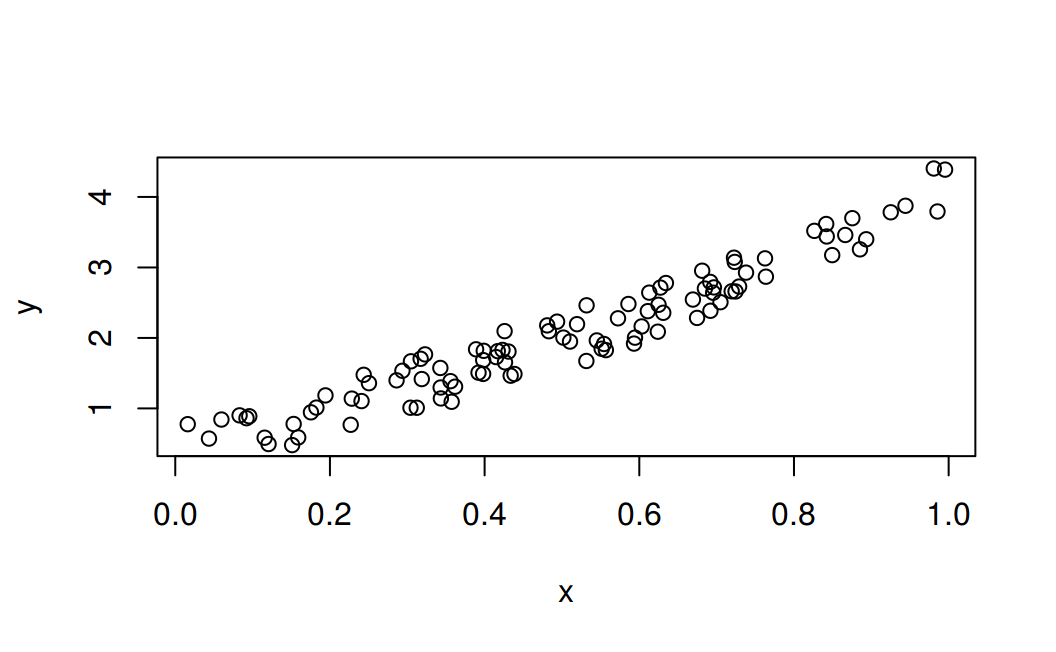
\includegraphics{rtorch-book_files/figure-latex/unnamed-chunk-56-1.pdf}

Before you start the training process, you need to convert the numpy array to Variables that supported by Torch and autograd.

\hypertarget{converting-from-numpy-to-tensor}{%
\subsection{Converting from numpy to tensor}\label{converting-from-numpy-to-tensor}}

Notice that before converting to a Torch tensor, we need first to convert the R numeric vector to a \texttt{numpy} array:

\begin{Shaded}
\begin{Highlighting}[]
\CommentTok{# convert numpy array to tensor in shape of input size}
\NormalTok{x <-}\StringTok{ }\KeywordTok{r_to_py}\NormalTok{(x)}
\NormalTok{y <-}\StringTok{ }\KeywordTok{r_to_py}\NormalTok{(y)}
\NormalTok{x =}\StringTok{ }\NormalTok{torch}\OperatorTok{$}\KeywordTok{from_numpy}\NormalTok{(x}\OperatorTok{$}\KeywordTok{reshape}\NormalTok{(}\OperatorTok{-}\NormalTok{1L, 1L))}\OperatorTok{$}\KeywordTok{float}\NormalTok{()}
\NormalTok{y =}\StringTok{ }\NormalTok{torch}\OperatorTok{$}\KeywordTok{from_numpy}\NormalTok{(y}\OperatorTok{$}\KeywordTok{reshape}\NormalTok{(}\OperatorTok{-}\NormalTok{1L, 1L))}\OperatorTok{$}\KeywordTok{float}\NormalTok{()}
\KeywordTok{print}\NormalTok{(x, y)}
\end{Highlighting}
\end{Shaded}

\begin{verbatim}
## tensor([[0.6965],
##         [0.2861],
##         [0.2269],
##         [0.5513],
##         [0.7195],
##         [0.4231],
##         [0.9808],
##         [0.6848],
##         [0.4809],
##         [0.3921],
##         [0.3432],
##         [0.7290],
##         [0.4386],
##         [0.0597],
##         [0.3980],
##         [0.7380],
##         [0.1825],
##         [0.1755],
##         [0.5316],
##         [0.5318],
##         [0.6344],
##         [0.8494],
##         [0.7245],
##         [0.6110],
##         [0.7224],
##         [0.3230],
##         [0.3618],
##         [0.2283],
##         [0.2937],
##         [0.6310],
##         [0.0921],
##         [0.4337],
##         [0.4309],
##         [0.4937],
##         [0.4258],
##         [0.3123],
##         [0.4264],
##         [0.8934],
##         [0.9442],
##         [0.5018],
##         [0.6240],
##         [0.1156],
##         [0.3173],
##         [0.4148],
##         [0.8663],
##         [0.2505],
##         [0.4830],
##         [0.9856],
##         [0.5195],
##         [0.6129],
##         [0.1206],
##         [0.8263],
##         [0.6031],
##         [0.5451],
##         [0.3428],
##         [0.3041],
##         [0.4170],
##         [0.6813],
##         [0.8755],
##         [0.5104],
##         [0.6693],
##         [0.5859],
##         [0.6249],
##         [0.6747],
##         [0.8423],
##         [0.0832],
##         [0.7637],
##         [0.2437],
##         [0.1942],
##         [0.5725],
##         [0.0957],
##         [0.8853],
##         [0.6272],
##         [0.7234],
##         [0.0161],
##         [0.5944],
##         [0.5568],
##         [0.1590],
##         [0.1531],
##         [0.6955],
##         [0.3188],
##         [0.6920],
##         [0.5544],
##         [0.3890],
##         [0.9251],
##         [0.8417],
##         [0.3574],
##         [0.0436],
##         [0.3048],
##         [0.3982],
##         [0.7050],
##         [0.9954],
##         [0.3559],
##         [0.7625],
##         [0.5932],
##         [0.6917],
##         [0.1511],
##         [0.3989],
##         [0.2409],
##         [0.3435]])
\end{verbatim}

\hypertarget{optimizer-and-loss}{%
\section{Optimizer and Loss}\label{optimizer-and-loss}}

Next, you should define the Optimizer and the Loss Function for our training process.

\begin{Shaded}
\begin{Highlighting}[]
\CommentTok{# Define Optimizer and Loss Function}
\NormalTok{optimizer <-}\StringTok{ }\NormalTok{torch}\OperatorTok{$}\NormalTok{optim}\OperatorTok{$}\KeywordTok{SGD}\NormalTok{(net}\OperatorTok{$}\KeywordTok{parameters}\NormalTok{(), }\DataTypeTok{lr=}\FloatTok{0.2}\NormalTok{)}
\NormalTok{loss_func <-}\StringTok{ }\NormalTok{torch}\OperatorTok{$}\NormalTok{nn}\OperatorTok{$}\KeywordTok{MSELoss}\NormalTok{()}
\KeywordTok{print}\NormalTok{(optimizer)}
\end{Highlighting}
\end{Shaded}

\begin{verbatim}
## SGD (
## Parameter Group 0
##     dampening: 0
##     lr: 0.2
##     momentum: 0
##     nesterov: False
##     weight_decay: 0
## )
\end{verbatim}

\begin{Shaded}
\begin{Highlighting}[]
\KeywordTok{print}\NormalTok{(loss_func)}
\end{Highlighting}
\end{Shaded}

\begin{verbatim}
## MSELoss()
\end{verbatim}

\hypertarget{training}{%
\section{Training}\label{training}}

Now let's start our training process. With an epoch of 250, you will iterate our data to find the best value for our hyperparameters.

\begin{Shaded}
\begin{Highlighting}[]
\CommentTok{# x = x$type(torch$float)   # make it a a FloatTensor}
\CommentTok{# y = y$type(torch$float)}

\CommentTok{# x <- torch$as_tensor(x, dtype = torch$float)}
\CommentTok{# y <- torch$as_tensor(y, dtype = torch$float)}

\NormalTok{inputs  =}\StringTok{ }\KeywordTok{Variable}\NormalTok{(x)}
\NormalTok{outputs =}\StringTok{ }\KeywordTok{Variable}\NormalTok{(y)}

\CommentTok{# base plot}
\KeywordTok{plot}\NormalTok{(x}\OperatorTok{$}\NormalTok{data}\OperatorTok{$}\KeywordTok{numpy}\NormalTok{(), y}\OperatorTok{$}\NormalTok{data}\OperatorTok{$}\KeywordTok{numpy}\NormalTok{(), }\DataTypeTok{col =} \StringTok{"blue"}\NormalTok{)}
\end{Highlighting}
\end{Shaded}

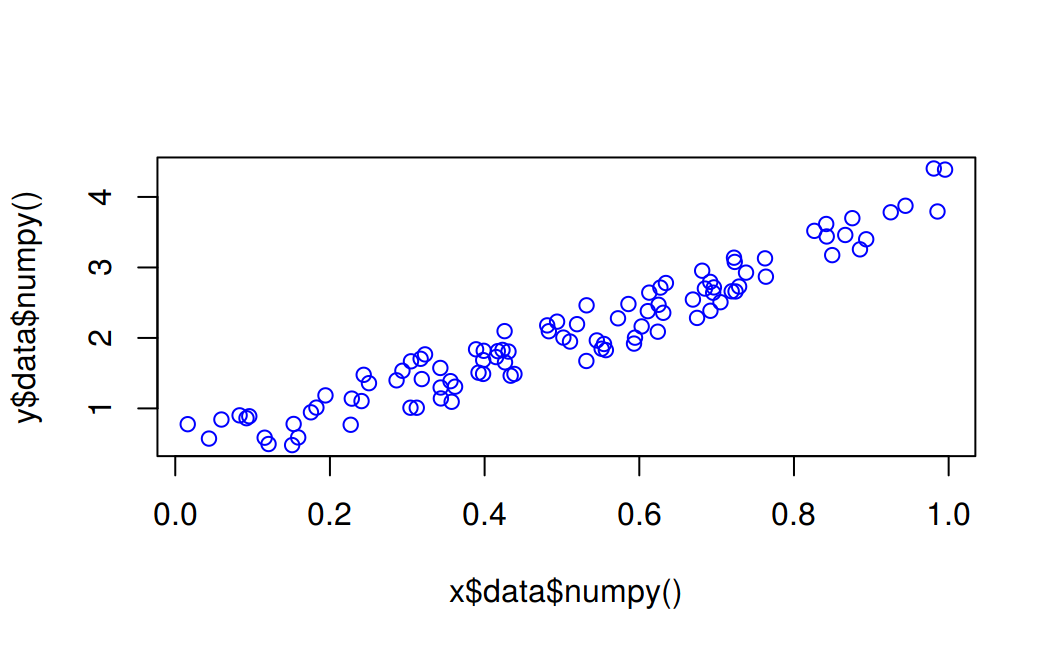
\includegraphics{rtorch-book_files/figure-latex/unnamed-chunk-59-1.pdf}

\begin{Shaded}
\begin{Highlighting}[]
\ControlFlowTok{for}\NormalTok{ (i }\ControlFlowTok{in} \DecValTok{1}\OperatorTok{:}\DecValTok{250}\NormalTok{) \{}
\NormalTok{   prediction =}\StringTok{ }\KeywordTok{net}\NormalTok{(inputs)}
\NormalTok{   loss =}\StringTok{ }\KeywordTok{loss_func}\NormalTok{(prediction, outputs)}
\NormalTok{   optimizer}\OperatorTok{$}\KeywordTok{zero_grad}\NormalTok{()}
\NormalTok{   loss}\OperatorTok{$}\KeywordTok{backward}\NormalTok{()}
\NormalTok{   optimizer}\OperatorTok{$}\KeywordTok{step}\NormalTok{()}
   
   \ControlFlowTok{if}\NormalTok{ (i }\OperatorTok{>}\StringTok{ }\DecValTok{1}\NormalTok{) }\ControlFlowTok{break}

   \ControlFlowTok{if}\NormalTok{ (i }\OperatorTok\StringTok{ }\DecValTok{10} \OperatorTok{==}\StringTok{ }\DecValTok{0}\NormalTok{) \{}
       \CommentTok{# plot and show learning process}
      \CommentTok{# points(x$data$numpy(), y$data$numpy())}
      \KeywordTok{points}\NormalTok{(x}\OperatorTok{$}\NormalTok{data}\OperatorTok{$}\KeywordTok{numpy}\NormalTok{(), prediction}\OperatorTok{$}\NormalTok{data}\OperatorTok{$}\KeywordTok{numpy}\NormalTok{(), }\DataTypeTok{col=}\StringTok{"red"}\NormalTok{)}
       \CommentTok{# cat(i, loss$data$numpy(), "\textbackslash{}n")}
\NormalTok{   \}}
\NormalTok{\}}
\end{Highlighting}
\end{Shaded}

\hypertarget{result}{%
\section{Result}\label{result}}

As you can see below, you successfully performed regression with a neural network. Actually, on every iteration, the red line in the plot will update and change its position to fit the data. But in this picture, you only show you the final result.

\hypertarget{case-2-rainfall}{%
\section{Case 2: Rainfall}\label{case-2-rainfall}}

\begin{Shaded}
\begin{Highlighting}[]
\KeywordTok{library}\NormalTok{(rTorch)}
\end{Highlighting}
\end{Shaded}

\hypertarget{select-device}{%
\section{Select device}\label{select-device}}

\begin{Shaded}
\begin{Highlighting}[]
\NormalTok{torch}\OperatorTok{$}\KeywordTok{manual_seed}\NormalTok{(}\DecValTok{0}\NormalTok{)}
\end{Highlighting}
\end{Shaded}

\begin{verbatim}
## <torch._C.Generator>
\end{verbatim}

\begin{Shaded}
\begin{Highlighting}[]
\NormalTok{device =}\StringTok{ }\NormalTok{torch}\OperatorTok{$}\KeywordTok{device}\NormalTok{(}\StringTok{'cpu'}\NormalTok{)}
\end{Highlighting}
\end{Shaded}

\hypertarget{training-data}{%
\section{Training data}\label{training-data}}

The training data can be represented using 2 matrices (inputs and targets), each with one row per observation, and one column per variable.

\begin{Shaded}
\begin{Highlighting}[]
\CommentTok{# Input (temp, rainfall, humidity)}
\NormalTok{inputs =}\StringTok{ }\NormalTok{np}\OperatorTok{$}\KeywordTok{array}\NormalTok{(}\KeywordTok{list}\NormalTok{(}\KeywordTok{list}\NormalTok{(}\DecValTok{73}\NormalTok{, }\DecValTok{67}\NormalTok{, }\DecValTok{43}\NormalTok{),}
                   \KeywordTok{list}\NormalTok{(}\DecValTok{91}\NormalTok{, }\DecValTok{88}\NormalTok{, }\DecValTok{64}\NormalTok{),}
                   \KeywordTok{list}\NormalTok{(}\DecValTok{87}\NormalTok{, }\DecValTok{134}\NormalTok{, }\DecValTok{58}\NormalTok{),}
                   \KeywordTok{list}\NormalTok{(}\DecValTok{102}\NormalTok{, }\DecValTok{43}\NormalTok{, }\DecValTok{37}\NormalTok{),}
                   \KeywordTok{list}\NormalTok{(}\DecValTok{69}\NormalTok{, }\DecValTok{96}\NormalTok{, }\DecValTok{70}\NormalTok{)), }\DataTypeTok{dtype=}\StringTok{'float32'}\NormalTok{)}

\CommentTok{# Targets (apples, oranges)}
\NormalTok{targets =}\StringTok{ }\NormalTok{np}\OperatorTok{$}\KeywordTok{array}\NormalTok{(}\KeywordTok{list}\NormalTok{(}\KeywordTok{list}\NormalTok{(}\DecValTok{56}\NormalTok{, }\DecValTok{70}\NormalTok{), }
                    \KeywordTok{list}\NormalTok{(}\DecValTok{81}\NormalTok{, }\DecValTok{101}\NormalTok{),}
                    \KeywordTok{list}\NormalTok{(}\DecValTok{119}\NormalTok{, }\DecValTok{133}\NormalTok{),}
                    \KeywordTok{list}\NormalTok{(}\DecValTok{22}\NormalTok{, }\DecValTok{37}\NormalTok{), }
                    \KeywordTok{list}\NormalTok{(}\DecValTok{103}\NormalTok{, }\DecValTok{119}\NormalTok{)), }\DataTypeTok{dtype=}\StringTok{'float32'}\NormalTok{)}
\end{Highlighting}
\end{Shaded}

\hypertarget{convert-to-tensors}{%
\section{Convert to tensors}\label{convert-to-tensors}}

Before we build a model, we need to convert inputs and targets to PyTorch tensors.

\begin{Shaded}
\begin{Highlighting}[]
\CommentTok{# Convert inputs and targets to tensors}
\NormalTok{inputs =}\StringTok{ }\NormalTok{torch}\OperatorTok{$}\KeywordTok{from_numpy}\NormalTok{(inputs)}
\NormalTok{targets =}\StringTok{ }\NormalTok{torch}\OperatorTok{$}\KeywordTok{from_numpy}\NormalTok{(targets)}

\KeywordTok{print}\NormalTok{(inputs)}
\end{Highlighting}
\end{Shaded}

\begin{verbatim}
## tensor([[ 73.,  67.,  43.],
##         [ 91.,  88.,  64.],
##         [ 87., 134.,  58.],
##         [102.,  43.,  37.],
##         [ 69.,  96.,  70.]], dtype=torch.float64)
\end{verbatim}

\begin{Shaded}
\begin{Highlighting}[]
\KeywordTok{print}\NormalTok{(targets)}
\end{Highlighting}
\end{Shaded}

\begin{verbatim}
## tensor([[ 56.,  70.],
##         [ 81., 101.],
##         [119., 133.],
##         [ 22.,  37.],
##         [103., 119.]], dtype=torch.float64)
\end{verbatim}

The weights and biases can also be represented as matrices, initialized with random values. The first row of \(w\) and the first element of \(b\) are used to predict the first target variable, i.e.~yield for apples, and, similarly, the second for oranges.

\begin{Shaded}
\begin{Highlighting}[]
\CommentTok{# random numbers for weights and biases. Then convert to double()}
\NormalTok{torch}\OperatorTok{$}\KeywordTok{set_default_dtype}\NormalTok{(torch}\OperatorTok{$}\NormalTok{double)}

\NormalTok{w =}\StringTok{ }\NormalTok{torch}\OperatorTok{$}\KeywordTok{randn}\NormalTok{(2L, 3L, }\DataTypeTok{requires_grad=}\OtherTok{TRUE}\NormalTok{)  }\CommentTok{#$double()}
\NormalTok{b =}\StringTok{ }\NormalTok{torch}\OperatorTok{$}\KeywordTok{randn}\NormalTok{(2L, }\DataTypeTok{requires_grad=}\OtherTok{TRUE}\NormalTok{)      }\CommentTok{#$double()}

\KeywordTok{print}\NormalTok{(w)}
\end{Highlighting}
\end{Shaded}

\begin{verbatim}
## tensor([[ 1.5410, -0.2934, -2.1788],
##         [ 0.5684, -1.0845, -1.3986]], requires_grad=True)
\end{verbatim}

\begin{Shaded}
\begin{Highlighting}[]
\KeywordTok{print}\NormalTok{(b)}
\end{Highlighting}
\end{Shaded}

\begin{verbatim}
## tensor([0.4033, 0.8380], requires_grad=True)
\end{verbatim}

\hypertarget{build-the-model}{%
\section{Build the model}\label{build-the-model}}

The model is simply a function that performs a matrix multiplication of the input \(x\) and the weights \(w\) (transposed), and adds the bias \(b\) (replicated for each observation).

\begin{Shaded}
\begin{Highlighting}[]
\NormalTok{model <-}\StringTok{ }\ControlFlowTok{function}\NormalTok{(x) \{}
\NormalTok{  wt <-}\StringTok{ }\NormalTok{w}\OperatorTok{$}\KeywordTok{t}\NormalTok{()}
  \KeywordTok{return}\NormalTok{(torch}\OperatorTok{$}\KeywordTok{add}\NormalTok{(torch}\OperatorTok{$}\KeywordTok{mm}\NormalTok{(x, wt), b))}
\NormalTok{\}}
\end{Highlighting}
\end{Shaded}

\hypertarget{generate-predictions}{%
\section{Generate predictions}\label{generate-predictions}}

The matrix obtained by passing the input data to the model is a set of predictions for the target variables.

\begin{Shaded}
\begin{Highlighting}[]
\CommentTok{# Generate predictions}
\NormalTok{preds =}\StringTok{ }\KeywordTok{model}\NormalTok{(inputs)}
\KeywordTok{print}\NormalTok{(preds)}
\end{Highlighting}
\end{Shaded}

\begin{verbatim}
## tensor([[  -0.4516,  -90.4691],
##         [ -24.6303, -132.3828],
##         [ -31.2192, -176.1530],
##         [  64.3523,  -39.5645],
##         [ -73.9524, -161.9560]], grad_fn=<AddBackward0>)
\end{verbatim}

\begin{Shaded}
\begin{Highlighting}[]
\CommentTok{# Compare with targets}
\KeywordTok{print}\NormalTok{(targets)}
\end{Highlighting}
\end{Shaded}

\begin{verbatim}
## tensor([[ 56.,  70.],
##         [ 81., 101.],
##         [119., 133.],
##         [ 22.,  37.],
##         [103., 119.]])
\end{verbatim}

Because we've started with random weights and biases, the model does not a very good job of predicting the target variables.

\hypertarget{loss-function}{%
\section{Loss Function}\label{loss-function}}

We can compare the predictions with the actual targets, using the following method:

\begin{itemize}
\tightlist
\item
  Calculate the difference between the two matrices (preds and targets).
\item
  Square all elements of the difference matrix to remove negative values.
\item
  Calculate the average of the elements in the resulting matrix.
\end{itemize}

The result is a single number, known as the mean squared error (MSE).

\begin{Shaded}
\begin{Highlighting}[]
\CommentTok{# MSE loss}
\NormalTok{mse =}\StringTok{ }\ControlFlowTok{function}\NormalTok{(t1, t2) \{}
\NormalTok{  diff <-}\StringTok{ }\NormalTok{torch}\OperatorTok{$}\KeywordTok{sub}\NormalTok{(t1, t2)}
\NormalTok{  mul <-}\StringTok{ }\NormalTok{torch}\OperatorTok{$}\KeywordTok{sum}\NormalTok{(torch}\OperatorTok{$}\KeywordTok{mul}\NormalTok{(diff, diff))}
  \KeywordTok{return}\NormalTok{(torch}\OperatorTok{$}\KeywordTok{div}\NormalTok{(mul, diff}\OperatorTok{$}\KeywordTok{numel}\NormalTok{()))}
\NormalTok{\}}
\end{Highlighting}
\end{Shaded}

\begin{Shaded}
\begin{Highlighting}[]
\CommentTok{# Compute loss}
\NormalTok{loss =}\StringTok{ }\KeywordTok{mse}\NormalTok{(preds, targets)}
\KeywordTok{print}\NormalTok{(loss)}
\end{Highlighting}
\end{Shaded}

\begin{verbatim}
## tensor(33060.8053, grad_fn=<DivBackward0>)
\end{verbatim}

\begin{Shaded}
\begin{Highlighting}[]
\CommentTok{# 46194}
\CommentTok{# 33060.8070}
\end{Highlighting}
\end{Shaded}

The resulting number is called the \textbf{loss}, because it indicates how bad the model is at predicting the target variables. Lower the loss, better the model.

\hypertarget{compute-gradients}{%
\section{Compute Gradients}\label{compute-gradients}}

With PyTorch, we can automatically compute the gradient or derivative of the loss w.r.t. to the weights and biases, because they have \texttt{requires\_grad} set to True.

\begin{Shaded}
\begin{Highlighting}[]
\CommentTok{# Compute gradients}
\NormalTok{loss}\OperatorTok{$}\KeywordTok{backward}\NormalTok{()}
\end{Highlighting}
\end{Shaded}

The gradients are stored in the .grad property of the respective tensors.

\begin{Shaded}
\begin{Highlighting}[]
\CommentTok{# Gradients for weights}
\KeywordTok{print}\NormalTok{(w)}
\end{Highlighting}
\end{Shaded}

\begin{verbatim}
## tensor([[ 1.5410, -0.2934, -2.1788],
##         [ 0.5684, -1.0845, -1.3986]], requires_grad=True)
\end{verbatim}

\begin{Shaded}
\begin{Highlighting}[]
\KeywordTok{print}\NormalTok{(w}\OperatorTok{$}\NormalTok{grad)}
\end{Highlighting}
\end{Shaded}

\begin{verbatim}
## tensor([[ -6938.4351,  -9674.6757,  -5744.0206],
##         [-17408.7861, -20595.9333, -12453.4702]])
\end{verbatim}

\begin{Shaded}
\begin{Highlighting}[]
\CommentTok{# Gradients for bias}
\KeywordTok{print}\NormalTok{(b)}
\end{Highlighting}
\end{Shaded}

\begin{verbatim}
## tensor([0.4033, 0.8380], requires_grad=True)
\end{verbatim}

\begin{Shaded}
\begin{Highlighting}[]
\KeywordTok{print}\NormalTok{(b}\OperatorTok{$}\NormalTok{grad)}
\end{Highlighting}
\end{Shaded}

\begin{verbatim}
## tensor([ -89.3802, -212.1051])
\end{verbatim}

A key insight from calculus is that the gradient indicates the rate of change of the loss, or the slope of the loss function w.r.t. the weights and biases.

\begin{itemize}
\tightlist
\item
  If a gradient element is positive:

  \begin{itemize}
  \tightlist
  \item
    increasing the element's value slightly will increase the loss.
  \item
    decreasing the element's value slightly will decrease the loss.
  \end{itemize}
\item
  If a gradient element is negative,

  \begin{itemize}
  \tightlist
  \item
    increasing the element's value slightly will decrease the loss.
  \item
    decreasing the element's value slightly will increase the loss.
  \end{itemize}
\end{itemize}

The increase or decrease is proportional to the value of the gradient.

Finally, we'll reset the gradients to zero before moving forward, because PyTorch accumulates gradients.

\begin{Shaded}
\begin{Highlighting}[]
\CommentTok{# Reset the gradients}
\NormalTok{w}\OperatorTok{$}\NormalTok{grad}\OperatorTok{$}\KeywordTok{zero_}\NormalTok{()}
\end{Highlighting}
\end{Shaded}

\begin{verbatim}
## tensor([[0., 0., 0.],
##         [0., 0., 0.]])
\end{verbatim}

\begin{Shaded}
\begin{Highlighting}[]
\NormalTok{b}\OperatorTok{$}\NormalTok{grad}\OperatorTok{$}\KeywordTok{zero_}\NormalTok{()}
\end{Highlighting}
\end{Shaded}

\begin{verbatim}
## tensor([0., 0.])
\end{verbatim}

\begin{Shaded}
\begin{Highlighting}[]
\KeywordTok{print}\NormalTok{(w}\OperatorTok{$}\NormalTok{grad)}
\end{Highlighting}
\end{Shaded}

\begin{verbatim}
## tensor([[0., 0., 0.],
##         [0., 0., 0.]])
\end{verbatim}

\begin{Shaded}
\begin{Highlighting}[]
\KeywordTok{print}\NormalTok{(b}\OperatorTok{$}\NormalTok{grad)}
\end{Highlighting}
\end{Shaded}

\begin{verbatim}
## tensor([0., 0.])
\end{verbatim}

\hypertarget{adjust-weights-and-biases-using-gradient-descent}{%
\section{Adjust weights and biases using gradient descent}\label{adjust-weights-and-biases-using-gradient-descent}}

We'll reduce the loss and improve our model using the gradient descent algorithm, which has the following steps:

\begin{enumerate}
\def\labelenumi{\arabic{enumi}.}
\tightlist
\item
  Generate predictions
\item
  Calculate the loss
\item
  Compute gradients w.r.t the weights and biases
\item
  Adjust the weights by subtracting a small quantity proportional to the gradient
\item
  Reset the gradients to zero
\end{enumerate}

\begin{Shaded}
\begin{Highlighting}[]
\CommentTok{# Generate predictions}
\NormalTok{preds =}\StringTok{ }\KeywordTok{model}\NormalTok{(inputs)}
\KeywordTok{print}\NormalTok{(preds)}
\end{Highlighting}
\end{Shaded}

\begin{verbatim}
## tensor([[  -0.4516,  -90.4691],
##         [ -24.6303, -132.3828],
##         [ -31.2192, -176.1530],
##         [  64.3523,  -39.5645],
##         [ -73.9524, -161.9560]], grad_fn=<AddBackward0>)
\end{verbatim}

\begin{Shaded}
\begin{Highlighting}[]
\CommentTok{# Calculate the loss}
\NormalTok{loss =}\StringTok{ }\KeywordTok{mse}\NormalTok{(preds, targets)}
\KeywordTok{print}\NormalTok{(loss)}
\end{Highlighting}
\end{Shaded}

\begin{verbatim}
## tensor(33060.8053, grad_fn=<DivBackward0>)
\end{verbatim}

\begin{Shaded}
\begin{Highlighting}[]
\CommentTok{# Compute gradients}
\NormalTok{loss}\OperatorTok{$}\KeywordTok{backward}\NormalTok{()}

\KeywordTok{print}\NormalTok{(w}\OperatorTok{$}\NormalTok{grad)}
\end{Highlighting}
\end{Shaded}

\begin{verbatim}
## tensor([[ -6938.4351,  -9674.6757,  -5744.0206],
##         [-17408.7861, -20595.9333, -12453.4702]])
\end{verbatim}

\begin{Shaded}
\begin{Highlighting}[]
\KeywordTok{print}\NormalTok{(b}\OperatorTok{$}\NormalTok{grad)}
\end{Highlighting}
\end{Shaded}

\begin{verbatim}
## tensor([ -89.3802, -212.1051])
\end{verbatim}

\begin{Shaded}
\begin{Highlighting}[]
\CommentTok{# Adjust weights and reset gradients}
\KeywordTok{with}\NormalTok{(torch}\OperatorTok{$}\KeywordTok{no_grad}\NormalTok{(), \{}
  \KeywordTok{print}\NormalTok{(w); }\KeywordTok{print}\NormalTok{(b)    }\CommentTok{# requires_grad attribute remains}
\NormalTok{  w}\OperatorTok{$}\NormalTok{data <-}\StringTok{ }\NormalTok{torch}\OperatorTok{$}\KeywordTok{sub}\NormalTok{(w}\OperatorTok{$}\NormalTok{data, torch}\OperatorTok{$}\KeywordTok{mul}\NormalTok{(w}\OperatorTok{$}\NormalTok{grad}\OperatorTok{$}\NormalTok{data, torch}\OperatorTok{$}\KeywordTok{scalar_tensor}\NormalTok{(}\FloatTok{1e-5}\NormalTok{)))}
\NormalTok{  b}\OperatorTok{$}\NormalTok{data <-}\StringTok{ }\NormalTok{torch}\OperatorTok{$}\KeywordTok{sub}\NormalTok{(b}\OperatorTok{$}\NormalTok{data, torch}\OperatorTok{$}\KeywordTok{mul}\NormalTok{(b}\OperatorTok{$}\NormalTok{grad}\OperatorTok{$}\NormalTok{data, torch}\OperatorTok{$}\KeywordTok{scalar_tensor}\NormalTok{(}\FloatTok{1e-5}\NormalTok{)))}

  \KeywordTok{print}\NormalTok{(w}\OperatorTok{$}\NormalTok{grad}\OperatorTok{$}\NormalTok{data}\OperatorTok{$}\KeywordTok{zero_}\NormalTok{())}
  \KeywordTok{print}\NormalTok{(b}\OperatorTok{$}\NormalTok{grad}\OperatorTok{$}\NormalTok{data}\OperatorTok{$}\KeywordTok{zero_}\NormalTok{())}
\NormalTok{\})}
\end{Highlighting}
\end{Shaded}

\begin{verbatim}
## tensor([[ 1.5410, -0.2934, -2.1788],
##         [ 0.5684, -1.0845, -1.3986]], requires_grad=True)
## tensor([0.4033, 0.8380], requires_grad=True)
## tensor([[0., 0., 0.],
##         [0., 0., 0.]])
## tensor([0., 0.])
\end{verbatim}

\begin{Shaded}
\begin{Highlighting}[]
\KeywordTok{print}\NormalTok{(w)}
\end{Highlighting}
\end{Shaded}

\begin{verbatim}
## tensor([[ 1.6104, -0.1967, -2.1213],
##         [ 0.7425, -0.8786, -1.2741]], requires_grad=True)
\end{verbatim}

\begin{Shaded}
\begin{Highlighting}[]
\KeywordTok{print}\NormalTok{(b)}
\end{Highlighting}
\end{Shaded}

\begin{verbatim}
## tensor([0.4042, 0.8401], requires_grad=True)
\end{verbatim}

With the new weights and biases, the model should have a lower loss.

\begin{Shaded}
\begin{Highlighting}[]
\CommentTok{# Calculate loss}
\NormalTok{preds =}\StringTok{ }\KeywordTok{model}\NormalTok{(inputs)}
\NormalTok{loss =}\StringTok{ }\KeywordTok{mse}\NormalTok{(preds, targets)}
\KeywordTok{print}\NormalTok{(loss)}
\end{Highlighting}
\end{Shaded}

\begin{verbatim}
## tensor(23432.4894, grad_fn=<DivBackward0>)
\end{verbatim}

\hypertarget{train-for-multiple-epochs}{%
\section{Train for multiple epochs}\label{train-for-multiple-epochs}}

To reduce the loss further, we repeat the process of adjusting the weights and biases using the gradients multiple times. Each iteration is called an \textbf{epoch}.

\begin{Shaded}
\begin{Highlighting}[]
\CommentTok{# Running all together}
\CommentTok{# Adjust weights and reset gradients}
\ControlFlowTok{for}\NormalTok{ (i }\ControlFlowTok{in} \DecValTok{1}\OperatorTok{:}\DecValTok{100}\NormalTok{) \{}
\NormalTok{  preds =}\StringTok{ }\KeywordTok{model}\NormalTok{(inputs)}
\NormalTok{  loss =}\StringTok{ }\KeywordTok{mse}\NormalTok{(preds, targets)}
\NormalTok{  loss}\OperatorTok{$}\KeywordTok{backward}\NormalTok{()}
  \KeywordTok{with}\NormalTok{(torch}\OperatorTok{$}\KeywordTok{no_grad}\NormalTok{(), \{}
\NormalTok{    w}\OperatorTok{$}\NormalTok{data <-}\StringTok{ }\NormalTok{torch}\OperatorTok{$}\KeywordTok{sub}\NormalTok{(w}\OperatorTok{$}\NormalTok{data, torch}\OperatorTok{$}\KeywordTok{mul}\NormalTok{(w}\OperatorTok{$}\NormalTok{grad, torch}\OperatorTok{$}\KeywordTok{scalar_tensor}\NormalTok{(}\FloatTok{1e-5}\NormalTok{)))}
\NormalTok{    b}\OperatorTok{$}\NormalTok{data <-}\StringTok{ }\NormalTok{torch}\OperatorTok{$}\KeywordTok{sub}\NormalTok{(b}\OperatorTok{$}\NormalTok{data, torch}\OperatorTok{$}\KeywordTok{mul}\NormalTok{(b}\OperatorTok{$}\NormalTok{grad, torch}\OperatorTok{$}\KeywordTok{scalar_tensor}\NormalTok{(}\FloatTok{1e-5}\NormalTok{)))}
    
\NormalTok{    w}\OperatorTok{$}\NormalTok{grad}\OperatorTok{$}\KeywordTok{zero_}\NormalTok{()}
\NormalTok{    b}\OperatorTok{$}\NormalTok{grad}\OperatorTok{$}\KeywordTok{zero_}\NormalTok{()}
\NormalTok{  \})}
\NormalTok{\}}

\CommentTok{# Calculate loss}
\NormalTok{preds =}\StringTok{ }\KeywordTok{model}\NormalTok{(inputs)}
\NormalTok{loss =}\StringTok{ }\KeywordTok{mse}\NormalTok{(preds, targets)}
\KeywordTok{print}\NormalTok{(loss)}
\end{Highlighting}
\end{Shaded}

\begin{verbatim}
## tensor(1258.0216, grad_fn=<DivBackward0>)
\end{verbatim}

\begin{Shaded}
\begin{Highlighting}[]
\CommentTok{# predictions}
\NormalTok{preds}
\end{Highlighting}
\end{Shaded}

\begin{verbatim}
## tensor([[ 69.2462,  80.2082],
##         [ 73.7183,  97.2052],
##         [118.5780, 124.9272],
##         [ 89.2282,  92.7052],
##         [ 47.4648,  80.7782]], grad_fn=<AddBackward0>)
\end{verbatim}

\begin{Shaded}
\begin{Highlighting}[]
\CommentTok{# Targets}
\NormalTok{targets}
\end{Highlighting}
\end{Shaded}

\begin{verbatim}
## tensor([[ 56.,  70.],
##         [ 81., 101.],
##         [119., 133.],
##         [ 22.,  37.],
##         [103., 119.]])
\end{verbatim}

\hypertarget{logistic-regression}{%
\chapter{Logistic Regression}\label{logistic-regression}}

\begin{Shaded}
\begin{Highlighting}[]
\KeywordTok{library}\NormalTok{(rTorch)}

\NormalTok{nn          <-}\StringTok{ }\NormalTok{torch}\OperatorTok{$}\NormalTok{nn}
\NormalTok{transforms  <-}\StringTok{ }\NormalTok{torchvision}\OperatorTok{$}\NormalTok{transforms}

\NormalTok{torch}\OperatorTok{$}\KeywordTok{set_default_dtype}\NormalTok{(torch}\OperatorTok{$}\NormalTok{float)}
\end{Highlighting}
\end{Shaded}

\hypertarget{hyperparameters}{%
\subsection{Hyperparameters}\label{hyperparameters}}

\begin{Shaded}
\begin{Highlighting}[]
\CommentTok{# Hyper-parameters }
\NormalTok{input_size    <-}\StringTok{ }\NormalTok{784L}
\NormalTok{num_classes   <-}\StringTok{ }\NormalTok{10L}
\NormalTok{num_epochs    <-}\StringTok{ }\NormalTok{5L}
\NormalTok{batch_size    <-}\StringTok{ }\NormalTok{100L}
\NormalTok{learning_rate <-}\StringTok{ }\FloatTok{0.001}
\end{Highlighting}
\end{Shaded}

\hypertarget{read-datasets}{%
\subsection{Read datasets}\label{read-datasets}}

\begin{Shaded}
\begin{Highlighting}[]
\CommentTok{# MNIST dataset (images and labels)}
\CommentTok{# IDX format}
\NormalTok{local_folder <-}\StringTok{ '../datasets/raw_data'}
\NormalTok{train_dataset =}\StringTok{ }\NormalTok{torchvision}\OperatorTok{$}\NormalTok{datasets}\OperatorTok{$}\KeywordTok{MNIST}\NormalTok{(}\DataTypeTok{root=}\NormalTok{local_folder, }
                                           \DataTypeTok{train=}\OtherTok{TRUE}\NormalTok{, }
                                           \DataTypeTok{transform=}\NormalTok{transforms}\OperatorTok{$}\KeywordTok{ToTensor}\NormalTok{(),}
                                           \DataTypeTok{download=}\OtherTok{TRUE}\NormalTok{)}

\NormalTok{test_dataset =}\StringTok{ }\NormalTok{torchvision}\OperatorTok{$}\NormalTok{datasets}\OperatorTok{$}\KeywordTok{MNIST}\NormalTok{(}\DataTypeTok{root=}\NormalTok{local_folder, }
                                          \DataTypeTok{train=}\OtherTok{FALSE}\NormalTok{, }
                                          \DataTypeTok{transform=}\NormalTok{transforms}\OperatorTok{$}\KeywordTok{ToTensor}\NormalTok{())}

\CommentTok{# Data loader (input pipeline)}
\NormalTok{train_loader =}\StringTok{ }\NormalTok{torch}\OperatorTok{$}\NormalTok{utils}\OperatorTok{$}\NormalTok{data}\OperatorTok{$}\KeywordTok{DataLoader}\NormalTok{(}\DataTypeTok{dataset=}\NormalTok{train_dataset, }
                                           \DataTypeTok{batch_size=}\NormalTok{batch_size, }
                                           \DataTypeTok{shuffle=}\OtherTok{TRUE}\NormalTok{)}

\NormalTok{test_loader =}\StringTok{ }\NormalTok{torch}\OperatorTok{$}\NormalTok{utils}\OperatorTok{$}\NormalTok{data}\OperatorTok{$}\KeywordTok{DataLoader}\NormalTok{(}\DataTypeTok{dataset=}\NormalTok{test_dataset, }
                                          \DataTypeTok{batch_size=}\NormalTok{batch_size, }
                                          \DataTypeTok{shuffle=}\OtherTok{FALSE}\NormalTok{)}
\end{Highlighting}
\end{Shaded}

\begin{Shaded}
\begin{Highlighting}[]
\KeywordTok{class}\NormalTok{(train_loader)}
\end{Highlighting}
\end{Shaded}

\begin{verbatim}
## [1] "torch.utils.data.dataloader.DataLoader"
## [2] "python.builtin.object"
\end{verbatim}

\begin{Shaded}
\begin{Highlighting}[]
\KeywordTok{length}\NormalTok{(train_loader)}
\end{Highlighting}
\end{Shaded}

\begin{verbatim}
## [1] 2
\end{verbatim}

\hypertarget{define-the-model}{%
\subsection{Define the model}\label{define-the-model}}

\begin{Shaded}
\begin{Highlighting}[]
\CommentTok{# Logistic regression model}
\NormalTok{model =}\StringTok{ }\NormalTok{nn}\OperatorTok{$}\KeywordTok{Linear}\NormalTok{(input_size, num_classes)}

\CommentTok{# Loss and optimizer}
\CommentTok{# nn.CrossEntropyLoss() computes softmax internally}
\NormalTok{criterion =}\StringTok{ }\NormalTok{nn}\OperatorTok{$}\KeywordTok{CrossEntropyLoss}\NormalTok{()  }
\NormalTok{optimizer =}\StringTok{ }\NormalTok{torch}\OperatorTok{$}\NormalTok{optim}\OperatorTok{$}\KeywordTok{SGD}\NormalTok{(model}\OperatorTok{$}\KeywordTok{parameters}\NormalTok{(), }\DataTypeTok{lr=}\NormalTok{learning_rate)  }
\KeywordTok{print}\NormalTok{(model)}
\end{Highlighting}
\end{Shaded}

\begin{verbatim}
## Linear(in_features=784, out_features=10, bias=True)
\end{verbatim}

\hypertarget{training-1}{%
\subsection{Training}\label{training-1}}

\begin{Shaded}
\begin{Highlighting}[]
\CommentTok{# Train the model}
\NormalTok{iter_train_loader <-}\StringTok{ }\KeywordTok{iterate}\NormalTok{(train_loader)}
\NormalTok{total_step <-}\KeywordTok{length}\NormalTok{(iter_train_loader)}
\end{Highlighting}
\end{Shaded}

\begin{Shaded}
\begin{Highlighting}[]
\ControlFlowTok{for}\NormalTok{ (epoch }\ControlFlowTok{in} \DecValTok{1}\OperatorTok{:}\NormalTok{num_epochs) \{}
\NormalTok{    i <-}\StringTok{  }\DecValTok{0}
    \ControlFlowTok{for}\NormalTok{ (obj }\ControlFlowTok{in}\NormalTok{ iter_train_loader) \{}
        
\NormalTok{        images <-}\StringTok{ }\NormalTok{obj[[}\DecValTok{1}\NormalTok{]]   }\CommentTok{# tensor torch.Size([64, 3, 28, 28])}
\NormalTok{        labels <-}\StringTok{ }\NormalTok{obj[[}\DecValTok{2}\NormalTok{]]   }\CommentTok{# tensor torch.Size([64]), labels from 0 to 9}
        \CommentTok{# cat(i, "\textbackslash{}t"); print(images$shape)}

        \CommentTok{# Reshape images to (batch_size, input_size)}
\NormalTok{        images <-}\StringTok{ }\NormalTok{images}\OperatorTok{$}\KeywordTok{reshape}\NormalTok{(}\OperatorTok{-}\NormalTok{1L, 28L}\OperatorTok{*}\NormalTok{28L)}
        \CommentTok{# images <- torch$as_tensor(images$reshape(-1L, 28L*28L), dtype=torch$double)}

        \CommentTok{# Forward pass}
\NormalTok{        outputs <-}\StringTok{ }\KeywordTok{model}\NormalTok{(images)}
\NormalTok{        loss <-}\StringTok{ }\KeywordTok{criterion}\NormalTok{(outputs, labels)}

        \CommentTok{# Backward and optimize}
\NormalTok{        optimizer}\OperatorTok{$}\KeywordTok{zero_grad}\NormalTok{()}
\NormalTok{        loss}\OperatorTok{$}\KeywordTok{backward}\NormalTok{()}
\NormalTok{        optimizer}\OperatorTok{$}\KeywordTok{step}\NormalTok{()}

        \ControlFlowTok{if}\NormalTok{ ((i}\OperatorTok{+}\DecValTok{1}\NormalTok{) }\OperatorTok\StringTok{ }\DecValTok{100} \OperatorTok{==}\StringTok{ }\DecValTok{0}\NormalTok{) \{}
            \KeywordTok{cat}\NormalTok{(}\KeywordTok{sprintf}\NormalTok{(}\StringTok{'Epoch [%d/%d], Step [%d/%d], Loss: %f }\CharTok{\textbackslash{}n}\StringTok{'}\NormalTok{,}
\NormalTok{                epoch}\OperatorTok{+}\DecValTok{1}\NormalTok{, num_epochs, i}\OperatorTok{+}\DecValTok{1}\NormalTok{, total_step, loss}\OperatorTok{$}\KeywordTok{item}\NormalTok{()))}
\NormalTok{        \}}
\NormalTok{        i <-}\StringTok{  }\NormalTok{i }\OperatorTok{+}\StringTok{ }\DecValTok{1}
\NormalTok{    \}}
\NormalTok{\}  }
\end{Highlighting}
\end{Shaded}

\begin{verbatim}
## Epoch [2/5], Step [100/600], Loss: 2.193622 
## Epoch [2/5], Step [200/600], Loss: 2.095055 
## Epoch [2/5], Step [300/600], Loss: 1.993158 
## Epoch [2/5], Step [400/600], Loss: 1.914482 
## Epoch [2/5], Step [500/600], Loss: 1.828060 
## Epoch [2/5], Step [600/600], Loss: 1.821115 
## Epoch [3/5], Step [100/600], Loss: 1.732071 
## Epoch [3/5], Step [200/600], Loss: 1.653721 
## Epoch [3/5], Step [300/600], Loss: 1.592439 
## Epoch [3/5], Step [400/600], Loss: 1.525097 
## Epoch [3/5], Step [500/600], Loss: 1.436987 
## Epoch [3/5], Step [600/600], Loss: 1.502717 
## Epoch [4/5], Step [100/600], Loss: 1.446447 
## Epoch [4/5], Step [200/600], Loss: 1.366274 
## Epoch [4/5], Step [300/600], Loss: 1.341085 
## Epoch [4/5], Step [400/600], Loss: 1.280446 
## Epoch [4/5], Step [500/600], Loss: 1.181919 
## Epoch [4/5], Step [600/600], Loss: 1.288031 
## Epoch [5/5], Step [100/600], Loss: 1.259706 
## Epoch [5/5], Step [200/600], Loss: 1.173801 
## Epoch [5/5], Step [300/600], Loss: 1.176926 
## Epoch [5/5], Step [400/600], Loss: 1.122017 
## Epoch [5/5], Step [500/600], Loss: 1.010820 
## Epoch [5/5], Step [600/600], Loss: 1.138838 
## Epoch [6/5], Step [100/600], Loss: 1.130953 
## Epoch [6/5], Step [200/600], Loss: 1.039641 
## Epoch [6/5], Step [300/600], Loss: 1.063141 
## Epoch [6/5], Step [400/600], Loss: 1.013657 
## Epoch [6/5], Step [500/600], Loss: 0.890745 
## Epoch [6/5], Step [600/600], Loss: 1.030636
\end{verbatim}

\hypertarget{prediction}{%
\subsection{Prediction}\label{prediction}}

\begin{Shaded}
\begin{Highlighting}[]
\CommentTok{# Adjust weights and reset gradients}
\NormalTok{iter_test_loader <-}\StringTok{ }\KeywordTok{iterate}\NormalTok{(test_loader)}

\KeywordTok{with}\NormalTok{(torch}\OperatorTok{$}\KeywordTok{no_grad}\NormalTok{(), \{}
\NormalTok{    correct <-}\StringTok{  }\DecValTok{0}
\NormalTok{    total <-}\StringTok{  }\DecValTok{0}
    \ControlFlowTok{for}\NormalTok{ (obj }\ControlFlowTok{in}\NormalTok{ iter_test_loader) \{}
\NormalTok{        images <-}\StringTok{ }\NormalTok{obj[[}\DecValTok{1}\NormalTok{]]   }\CommentTok{# tensor torch.Size([64, 3, 28, 28])}
\NormalTok{        labels <-}\StringTok{ }\NormalTok{obj[[}\DecValTok{2}\NormalTok{]]   }\CommentTok{# tensor torch.Size([64]), labels from 0 to 9}
\NormalTok{        images =}\StringTok{ }\NormalTok{images}\OperatorTok{$}\KeywordTok{reshape}\NormalTok{(}\OperatorTok{-}\NormalTok{1L, 28L}\OperatorTok{*}\NormalTok{28L)}
        \CommentTok{# images <- torch$as_tensor(images$reshape(-1L, 28L*28L), dtype=torch$double)}
\NormalTok{        outputs =}\StringTok{ }\KeywordTok{model}\NormalTok{(images)}
\NormalTok{        .predicted =}\StringTok{ }\NormalTok{torch}\OperatorTok{$}\KeywordTok{max}\NormalTok{(outputs}\OperatorTok{$}\NormalTok{data, 1L)}
\NormalTok{        predicted <-}\StringTok{ }\NormalTok{.predicted[1L]}
\NormalTok{        total =}\StringTok{ }\NormalTok{total }\OperatorTok{+}\StringTok{ }\NormalTok{labels}\OperatorTok{$}\KeywordTok{size}\NormalTok{(0L)}
\NormalTok{        correct =}\StringTok{ }\NormalTok{correct }\OperatorTok{+}\StringTok{ }\KeywordTok{sum}\NormalTok{((predicted}\OperatorTok{$}\KeywordTok{numpy}\NormalTok{() }\OperatorTok{==}\StringTok{ }\NormalTok{labels}\OperatorTok{$}\KeywordTok{numpy}\NormalTok{()))}
\NormalTok{    \}}
    \KeywordTok{cat}\NormalTok{(}\KeywordTok{sprintf}\NormalTok{(}\StringTok{'Accuracy of the model on the 10000 test images: %f %%'}\NormalTok{, (}\DecValTok{100} \OperatorTok{*}\StringTok{ }\NormalTok{correct }\OperatorTok{/}\StringTok{ }\NormalTok{total)))}
  
\NormalTok{\})}
\end{Highlighting}
\end{Shaded}

\begin{verbatim}
## Accuracy of the model on the 10000 test images: 83.730000 %
\end{verbatim}

\hypertarget{save-the-model}{%
\subsection{Save the model}\label{save-the-model}}

\begin{Shaded}
\begin{Highlighting}[]
\CommentTok{# Save the model checkpoint}
\NormalTok{torch}\OperatorTok{$}\KeywordTok{save}\NormalTok{(model}\OperatorTok{$}\KeywordTok{state_dict}\NormalTok{(), }\StringTok{'model.ckpt'}\NormalTok{)}
\end{Highlighting}
\end{Shaded}

\hypertarget{neural-networks}{%
\chapter{Neural Networks}\label{neural-networks}}

Source: \url{https://github.com/jcjohnson/pytorch-examples\#pytorch-nn}

In this example we use the torch \texttt{nn} package to implement our two-layer network:

\hypertarget{in-r}{%
\section{In R}\label{in-r}}

\hypertarget{select-device-1}{%
\subsection{Select device}\label{select-device-1}}

\begin{Shaded}
\begin{Highlighting}[]
\KeywordTok{library}\NormalTok{(rTorch)}

\NormalTok{device =}\StringTok{ }\NormalTok{torch}\OperatorTok{$}\KeywordTok{device}\NormalTok{(}\StringTok{'cpu'}\NormalTok{)}

\CommentTok{# device = torch.device('cuda') # Uncomment this to run on GPU}
\end{Highlighting}
\end{Shaded}

\begin{verbatim}
 N is batch size; 
 D_in is input dimension;
 H is hidden dimension; 
 D_out is output dimension.
\end{verbatim}

\hypertarget{create-datasets}{%
\subsection{Create datasets}\label{create-datasets}}

\begin{Shaded}
\begin{Highlighting}[]
\NormalTok{torch}\OperatorTok{$}\KeywordTok{manual_seed}\NormalTok{(}\DecValTok{0}\NormalTok{)}
\end{Highlighting}
\end{Shaded}

\begin{verbatim}
## <torch._C.Generator>
\end{verbatim}

\begin{Shaded}
\begin{Highlighting}[]
\NormalTok{N <-}\StringTok{ }\NormalTok{64L; D_in <-}\StringTok{ }\NormalTok{1000L; H <-}\StringTok{ }\NormalTok{100L; D_out <-}\StringTok{ }\NormalTok{10L}

\CommentTok{# Create random Tensors to hold inputs and outputs}
\NormalTok{x =}\StringTok{ }\NormalTok{torch}\OperatorTok{$}\KeywordTok{randn}\NormalTok{(N, D_in, }\DataTypeTok{device=}\NormalTok{device)}
\NormalTok{y =}\StringTok{ }\NormalTok{torch}\OperatorTok{$}\KeywordTok{randn}\NormalTok{(N, D_out, }\DataTypeTok{device=}\NormalTok{device)}
\end{Highlighting}
\end{Shaded}

\hypertarget{define-the-model-1}{%
\subsection{Define the model}\label{define-the-model-1}}

Use the \texttt{nn} package to define our model as a sequence of layers. \texttt{nn.Sequential}
is a Module which contains other Modules, and applies them in sequence to
produce its output. Each Linear Module computes output from input using a
linear function, and holds internal Tensors for its weight and bias.
After constructing the model we use the \texttt{.to()} method to move it to the
desired device.

\begin{Shaded}
\begin{Highlighting}[]
\NormalTok{model =}\StringTok{ }\NormalTok{torch}\OperatorTok{$}\NormalTok{nn}\OperatorTok{$}\KeywordTok{Sequential}\NormalTok{(}
\NormalTok{          torch}\OperatorTok{$}\NormalTok{nn}\OperatorTok{$}\KeywordTok{Linear}\NormalTok{(D_in, H),}
\NormalTok{          torch}\OperatorTok{$}\NormalTok{nn}\OperatorTok{$}\KeywordTok{ReLU}\NormalTok{(),}
\NormalTok{          torch}\OperatorTok{$}\NormalTok{nn}\OperatorTok{$}\KeywordTok{Linear}\NormalTok{(H, D_out))}\OperatorTok{$}\KeywordTok{to}\NormalTok{(device)}
\end{Highlighting}
\end{Shaded}

\hypertarget{loss-function-1}{%
\subsection{Loss function}\label{loss-function-1}}

The \texttt{nn} package also contains definitions of popular loss functions; in this case we will use Mean Squared Error (MSE) as our loss function. Setting \texttt{reduction=\textquotesingle{}sum\textquotesingle{}} means that we are computing the \emph{sum} of squared errors rather than the mean; this is for consistency with the examples above where we manually compute the loss, but in practice it is more common to use mean squared error as a loss by setting \texttt{reduction=\textquotesingle{}elementwise\_mean\textquotesingle{}}.

\begin{Shaded}
\begin{Highlighting}[]
\NormalTok{loss_fn =}\StringTok{ }\NormalTok{torch}\OperatorTok{$}\NormalTok{nn}\OperatorTok{$}\KeywordTok{MSELoss}\NormalTok{(}\DataTypeTok{reduction =} \StringTok{'sum'}\NormalTok{)}
\end{Highlighting}
\end{Shaded}

\hypertarget{iterate-through-batches}{%
\subsection{Iterate through batches}\label{iterate-through-batches}}

\begin{Shaded}
\begin{Highlighting}[]
\NormalTok{learning_rate =}\StringTok{ }\FloatTok{1e-4}

\ControlFlowTok{for}\NormalTok{ (t }\ControlFlowTok{in} \DecValTok{1}\OperatorTok{:}\DecValTok{500}\NormalTok{) \{}
  \CommentTok{# Forward pass: compute predicted y by passing x to the model. Module objects}
  \CommentTok{# override the __call__ operator so you can call them like functions. When}
  \CommentTok{# doing so you pass a Tensor of input data to the Module and it produces}
  \CommentTok{# a Tensor of output data.}
\NormalTok{  y_pred =}\StringTok{ }\KeywordTok{model}\NormalTok{(x)}

  \CommentTok{# Compute and print loss. We pass Tensors containing the predicted and true}
  \CommentTok{# values of y, and the loss function returns a Tensor containing the loss.}
\NormalTok{  loss =}\StringTok{ }\KeywordTok{loss_fn}\NormalTok{(y_pred, y)}
  
  \KeywordTok{cat}\NormalTok{(t, }\StringTok{"}\CharTok{\textbackslash{}t}\StringTok{"}\NormalTok{)}
  \KeywordTok{cat}\NormalTok{(loss}\OperatorTok{$}\KeywordTok{item}\NormalTok{(), }\StringTok{"}\CharTok{\textbackslash{}n}\StringTok{"}\NormalTok{)}
  
  \CommentTok{# Zero the gradients before running the backward pass.}
\NormalTok{  model}\OperatorTok{$}\KeywordTok{zero_grad}\NormalTok{()}

  \CommentTok{# Backward pass: compute gradient of the loss with respect to all the learnable}
  \CommentTok{# parameters of the model. Internally, the parameters of each Module are stored}
  \CommentTok{# in Tensors with requires_grad=True, so this call will compute gradients for}
  \CommentTok{# all learnable parameters in the model.}
\NormalTok{  loss}\OperatorTok{$}\KeywordTok{backward}\NormalTok{()}

  \CommentTok{# Update the weights using gradient descent. Each parameter is a Tensor, so}
  \CommentTok{# we can access its data and gradients like we did before.}
  \KeywordTok{with}\NormalTok{(torch}\OperatorTok{$}\KeywordTok{no_grad}\NormalTok{(), \{}
      \ControlFlowTok{for}\NormalTok{ (param }\ControlFlowTok{in} \KeywordTok{iterate}\NormalTok{(model}\OperatorTok{$}\KeywordTok{parameters}\NormalTok{())) \{}
        \CommentTok{# in Python this code is much simpler. In R we have to do some conversions}
        
        \CommentTok{# param$data <- torch$sub(param$data,}
        \CommentTok{#                         torch$mul(param$grad$float(),}
        \CommentTok{#                           torch$scalar_tensor(learning_rate)))}
        
\NormalTok{        param}\OperatorTok{$}\NormalTok{data <-}\StringTok{ }\NormalTok{param}\OperatorTok{$}\NormalTok{data }\OperatorTok{-}\StringTok{ }\NormalTok{param}\OperatorTok{$}\NormalTok{grad }\OperatorTok{*}\StringTok{ }\NormalTok{learning_rate}
\NormalTok{      \}}
\NormalTok{   \})}
\NormalTok{\}  }
\end{Highlighting}
\end{Shaded}

\begin{verbatim}
## 1    628.2839 
## 2    584.9592 
## 3    546.728 
## 4    512.6885 
## 5    482.1306 
## 6    454.6265 
## 7    429.5551 
## 8    406.399 
## 9    384.6441 
## 10   364.3125 
## 11   345.3866 
## 12   327.6258 
## 13   310.8002 
## 14   294.8379 
## 15   279.7325 
## 16   265.308 
## 17   251.6231 
## 18   238.5361 
## 19   226.0232 
## 20   214.1025 
## 21   202.7003 
## 22   191.8059 
## 23   181.4473 
## 24   171.5948 
## 25   162.2114 
## 26   153.2922 
## 27   144.8526 
## 28   136.86 
## 29   129.2786 
## 30   122.0849 
## 31   115.2736 
## 32   108.8145 
## 33   102.702 
## 34   96.9281 
## 35   91.47466 
## 36   86.3278 
## 37   81.47502 
## 38   76.89146 
## 39   72.56895 
## 40   68.47774 
## 41   64.62608 
## 42   60.99714 
## 43   57.56915 
## 44   54.3427 
## 45   51.30913 
## 46   48.4516 
## 47   45.7645 
## 48   43.2405 
## 49   40.86606 
## 50   38.63006 
## 51   36.52527 
## 52   34.54914 
## 53   32.69345 
## 54   30.9498 
## 55   29.30734 
## 56   27.76275 
## 57   26.31089 
## 58   24.9431 
## 59   23.6538 
## 60   22.43881 
## 61   21.29258 
## 62   20.21278 
## 63   19.19288 
## 64   18.23302 
## 65   17.32939 
## 66   16.47696 
## 67   15.67115 
## 68   14.90951 
## 69   14.19054 
## 70   13.51087 
## 71   12.86819 
## 72   12.26046 
## 73   11.68514 
## 74   11.14105 
## 75   10.62579 
## 76   10.13727 
## 77   9.67443 
## 78   9.235745 
## 79   8.81936 
## 80   8.423415 
## 81   8.047976 
## 82   7.691305 
## 83   7.352424 
## 84   7.030395 
## 85   6.724676 
## 86   6.434433 
## 87   6.158278 
## 88   5.895441 
## 89   5.645772 
## 90   5.408593 
## 91   5.182788 
## 92   4.967783 
## 93   4.762821 
## 94   4.567942 
## 95   4.381676 
## 96   4.203955 
## 97   4.034254 
## 98   3.872373 
## 99   3.717669 
## 100  3.569852 
## 101  3.42879 
## 102  3.293934 
## 103  3.165006 
## 104  3.041733 
## 105  2.923832 
## 106  2.810992 
## 107  2.702966 
## 108  2.599546 
## 109  2.500533 
## 110  2.405609 
## 111  2.314677 
## 112  2.227567 
## 113  2.143984 
## 114  2.063824 
## 115  1.986898 
## 116  1.913161 
## 117  1.842398 
## 118  1.77456 
## 119  1.709334 
## 120  1.64675 
## 121  1.586662 
## 122  1.528932 
## 123  1.473498 
## 124  1.420194 
## 125  1.369045 
## 126  1.319939 
## 127  1.272713 
## 128  1.227352 
## 129  1.183716 
## 130  1.141713 
## 131  1.101289 
## 132  1.062379 
## 133  1.024975 
## 134  0.9889802 
## 135  0.9543175 
## 136  0.9209599 
## 137  0.8888108 
## 138  0.8578573 
## 139  0.828075 
## 140  0.7993811 
## 141  0.7717422 
## 142  0.7451235 
## 143  0.7194628 
## 144  0.6947174 
## 145  0.6708718 
## 146  0.6479479 
## 147  0.6259133 
## 148  0.6046655 
## 149  0.5841969 
## 150  0.5644467 
## 151  0.5453879 
## 152  0.5270226 
## 153  0.509312 
## 154  0.4922202 
## 155  0.4757309 
## 156  0.4598286 
## 157  0.444492 
## 158  0.4296912 
## 159  0.4153878 
## 160  0.4015924 
## 161  0.3882794 
## 162  0.3754345 
## 163  0.3630294 
## 164  0.3510535 
## 165  0.3394946 
## 166  0.3283299 
## 167  0.3175527 
## 168  0.3071378 
## 169  0.2970789 
## 170  0.2873671 
## 171  0.2779845 
## 172  0.2689149 
## 173  0.2601575 
## 174  0.2516952 
## 175  0.2435159 
## 176  0.2356067 
## 177  0.2279707 
## 178  0.2206163 
## 179  0.2135031 
## 180  0.2066278 
## 181  0.199988 
## 182  0.1935741 
## 183  0.1873666 
## 184  0.1813661 
## 185  0.1755629 
## 186  0.1699517 
## 187  0.1645233 
## 188  0.1592781 
## 189  0.1542067 
## 190  0.149301 
## 191  0.1445545 
## 192  0.1399648 
## 193  0.1355246 
## 194  0.1312279 
## 195  0.1270718 
## 196  0.1230509 
## 197  0.1191625 
## 198  0.115399 
## 199  0.1117588 
## 200  0.1082348 
## 201  0.1048254 
## 202  0.1015256 
## 203  0.09833349 
## 204  0.09524446 
## 205  0.0922533 
## 206  0.08935806 
## 207  0.08655693 
## 208  0.08384982 
## 209  0.081232 
## 210  0.07869583 
## 211  0.07624327 
## 212  0.0738695 
## 213  0.07157086 
## 214  0.06934651 
## 215  0.0671912 
## 216  0.06510548 
## 217  0.0630878 
## 218  0.0611335 
## 219  0.05924014 
## 220  0.05740607 
## 221  0.05563042 
## 222  0.05391053 
## 223  0.05224558 
## 224  0.05063397 
## 225  0.04907332 
## 226  0.04756238 
## 227  0.04609917 
## 228  0.0446822 
## 229  0.04330759 
## 230  0.04197593 
## 231  0.04068634 
## 232  0.03943768 
## 233  0.03822812 
## 234  0.0370564 
## 235  0.03592146 
## 236  0.03482136 
## 237  0.03375633 
## 238  0.0327246 
## 239  0.03172487 
## 240  0.03075593 
## 241  0.02981687 
## 242  0.02890735 
## 243  0.02802622 
## 244  0.02717285 
## 245  0.02634558 
## 246  0.02554371 
## 247  0.02476675 
## 248  0.0240143 
## 249  0.02328515 
## 250  0.02257836 
## 251  0.02189306 
## 252  0.02122923 
## 253  0.02058575 
## 254  0.01996238 
## 255  0.01935788 
## 256  0.01877213 
## 257  0.01820429 
## 258  0.01765402 
## 259  0.01712051 
## 260  0.01660351 
## 261  0.01610242 
## 262  0.0156171 
## 263  0.01514632 
## 264  0.01469009 
## 265  0.01424752 
## 266  0.01381863 
## 267  0.01340292 
## 268  0.01299987 
## 269  0.01260905 
## 270  0.01223013 
## 271  0.01186274 
## 272  0.01150682 
## 273  0.0111617 
## 274  0.01082683 
## 275  0.01050223 
## 276  0.01018802 
## 277  0.009882836 
## 278  0.009586995 
## 279  0.009300183 
## 280  0.009021979 
## 281  0.008752229 
## 282  0.008490788 
## 283  0.008237117 
## 284  0.007991165 
## 285  0.007752791 
## 286  0.007521485 
## 287  0.00729729 
## 288  0.0070798 
## 289  0.006868829 
## 290  0.006664461 
## 291  0.006466233 
## 292  0.006273943 
## 293  0.006087383 
## 294  0.005906438 
## 295  0.005730878 
## 296  0.005560733 
## 297  0.005395614 
## 298  0.005235502 
## 299  0.005080266 
## 300  0.004929713 
## 301  0.004783633 
## 302  0.004641939 
## 303  0.004504489 
## 304  0.004371175 
## 305  0.004241788 
## 306  0.004116328 
## 307  0.003994633 
## 308  0.003876575 
## 309  0.003762146 
## 310  0.003650998 
## 311  0.003543299 
## 312  0.003438761 
## 313  0.003337309 
## 314  0.003238867 
## 315  0.0031434 
## 316  0.003050815 
## 317  0.002960989 
## 318  0.002873863 
## 319  0.002789256 
## 320  0.002707202 
## 321  0.002627575 
## 322  0.002550329 
## 323  0.002475383 
## 324  0.002402639 
## 325  0.002332083 
## 326  0.002263665 
## 327  0.002197253 
## 328  0.0021328 
## 329  0.002070281 
## 330  0.002009582 
## 331  0.001950708 
## 332  0.001893577 
## 333  0.001838136 
## 334  0.001784306 
## 335  0.001732112 
## 336  0.001681432 
## 337  0.0016323 
## 338  0.001584614 
## 339  0.001538318 
## 340  0.00149336 
## 341  0.001449755 
## 342  0.001407453 
## 343  0.001366422 
## 344  0.001326558 
## 345  0.001287868 
## 346  0.001250318 
## 347  0.001213876 
## 348  0.00117851 
## 349  0.0011442 
## 350  0.001110891 
## 351  0.001078564 
## 352  0.001047205 
## 353  0.001016748 
## 354  0.000987183 
## 355  0.0009584787 
## 356  0.0009306203 
## 357  0.0009035908 
## 358  0.0008773552 
## 359  0.0008518948 
## 360  0.0008271908 
## 361  0.0008032027 
## 362  0.0007798997 
## 363  0.0007572919 
## 364  0.0007353517 
## 365  0.0007140448 
## 366  0.0006933782 
## 367  0.0006733016 
## 368  0.0006538091 
## 369  0.0006348886 
## 370  0.0006165295 
## 371  0.0005986958 
## 372  0.0005813859 
## 373  0.0005645752 
## 374  0.0005482732 
## 375  0.0005324451 
## 376  0.0005170752 
## 377  0.00050215 
## 378  0.0004876566 
## 379  0.0004735905 
## 380  0.0004599217 
## 381  0.000446661 
## 382  0.0004337932 
## 383  0.000421295 
## 384  0.000409168 
## 385  0.000397383 
## 386  0.0003859476 
## 387  0.0003748359 
## 388  0.000364068 
## 389  0.0003535805 
## 390  0.0003434142 
## 391  0.0003335507 
## 392  0.0003239612 
## 393  0.0003146584 
## 394  0.0003056151 
## 395  0.0002968509 
## 396  0.0002883257 
## 397  0.0002800551 
## 398  0.0002720189 
## 399  0.000264218 
## 400  0.0002566472 
## 401  0.0002492882 
## 402  0.0002421443 
## 403  0.0002352033 
## 404  0.000228468 
## 405  0.000221927 
## 406  0.0002155735 
## 407  0.000209406 
## 408  0.0002034151 
## 409  0.0001976036 
## 410  0.0001919538 
## 411  0.000186465 
## 412  0.000181138 
## 413  0.0001759652 
## 414  0.0001709464 
## 415  0.0001660616 
## 416  0.0001613203 
## 417  0.0001567196 
## 418  0.0001522457 
## 419  0.0001479028 
## 420  0.0001436849 
## 421  0.0001395875 
## 422  0.0001356086 
## 423  0.0001317492 
## 424  0.0001279981 
## 425  0.0001243516 
## 426  0.0001208117 
## 427  0.0001173674 
## 428  0.0001140324 
## 429  0.0001107887 
## 430  0.0001076371 
## 431  0.000104577 
## 432  0.0001016119 
## 433  9.872603e-05 
## 434  9.591727e-05 
## 435  9.320263e-05 
## 436  9.055879e-05 
## 437  8.798708e-05 
## 438  8.549038e-05 
## 439  8.306588e-05 
## 440  8.071403e-05 
## 441  7.842657e-05 
## 442  7.62079e-05 
## 443  7.40515e-05 
## 444  7.195051e-05 
## 445  6.991543e-05 
## 446  6.79373e-05 
## 447  6.601425e-05 
## 448  6.414913e-05 
## 449  6.233487e-05 
## 450  6.057473e-05 
## 451  5.886107e-05 
## 452  5.719856e-05 
## 453  5.558319e-05 
## 454  5.401246e-05 
## 455  5.24875e-05 
## 456  5.100614e-05 
## 457  4.957083e-05 
## 458  4.817137e-05 
## 459  4.681194e-05 
## 460  4.549512e-05 
## 461  4.420892e-05 
## 462  4.296327e-05 
## 463  4.175395e-05 
## 464  4.057565e-05 
## 465  3.943508e-05 
## 466  3.832371e-05 
## 467  3.724535e-05 
## 468  3.619579e-05 
## 469  3.517841e-05 
## 470  3.419127e-05 
## 471  3.322741e-05 
## 472  3.229243e-05 
## 473  3.138653e-05 
## 474  3.050298e-05 
## 475  2.964781e-05 
## 476  2.881304e-05 
## 477  2.800681e-05 
## 478  2.721956e-05 
## 479  2.645602e-05 
## 480  2.57129e-05 
## 481  2.499174e-05 
## 482  2.429051e-05 
## 483  2.361012e-05 
## 484  2.294818e-05 
## 485  2.230642e-05 
## 486  2.167962e-05 
## 487  2.107264e-05 
## 488  2.048336e-05 
## 489  1.991114e-05 
## 490  1.935353e-05 
## 491  1.88103e-05 
## 492  1.82841e-05 
## 493  1.777284e-05 
## 494  1.727619e-05 
## 495  1.67922e-05 
## 496  1.632309e-05 
## 497  1.586889e-05 
## 498  1.54238e-05 
## 499  1.499398e-05 
## 500  1.457493e-05
\end{verbatim}

These two expression are equivalent, with the first being the long version natural way of doing it in PyTorch. The second is using the generics in R for subtraction, multiplication and scalar conversion.

\begin{verbatim}
param$data <- torch$sub(param$data,
                        torch$mul(param$grad$float(),
                          torch$scalar_tensor(learning_rate)))
}
\end{verbatim}

\begin{verbatim}
param$data <- param$data - param$grad * learning_rate
\end{verbatim}

\hypertarget{datasets-in-pytorch}{%
\chapter{Datasets in PyTorch}\label{datasets-in-pytorch}}

\bibliography{book.bib,packages.bib}


\end{document}
